\documentclass[a4paper,12pt]{article}
\usepackage{latexsym}
\usepackage{array}
\usepackage{amsmath}
\usepackage{amsfonts}
\usepackage{bm}
\usepackage{color}
\usepackage{colortbl}
\usepackage{cite}
\usepackage{float}
\usepackage{graphicx}
\usepackage{ulem}
\usepackage{booktabs}
\usepackage[Symbol]{upgreek}
\usepackage{subfigure}
\usepackage{stfloats}
\usepackage{threeparttable}
\usepackage{theorem}
\usepackage{times}
\usepackage{dcolumn}
\usepackage{multirow}
\usepackage[boxed]{algorithm2e}
\usepackage{framed}

\newtheorem{theorem}{\bf Theorem}
\newtheorem{proposition}{\bf Proposition}
\newtheorem{lemma}{\bf Lemma}
\newtheorem{definition}{Definition}
\newtheorem{remark}{\bf Remark}


\setlength{\textheight}{245mm}
\setlength{\textwidth}{170mm}
\setlength{\topmargin}{-15mm}
\setlength{\oddsidemargin}{-5mm}
\setlength{\evensidemargin}{-5mm}
\flushbottom
\setlength{\parindent}{0pt}
\setlength{\baselineskip}{17pt}
\setlength{\parskip}{3mm}
\setlength{\columnsep}{8mm}
\renewcommand{\baselinestretch}{1.65}
\hyphenation{op-tical net-works semi-conduc-tor IEEEtran}
\DeclareGraphicsRule{.png}{eps}{.bb}{}

\newcommand{\PreserveBackslash}[1]{\let\temp=\\#1\let\\=\temp}
\newcommand{\red}[1]{\textcolor{red}{#1}}
\newcommand{\blue}[1]{\textcolor{blue}{#1}}


\newcolumntype{C}[1]{>{\PreserveBackslash\centering}p{#1}}
\newcolumntype{R}[1]{>{\PreserveBackslash\raggedleft}p{#1}}
\newcolumntype{L}[1]{>{\PreserveBackslash\raggedright}p{#1}}

\def \T {^{\mathsf{T}}}
\def \H {^{\mathsf{H}}}
\def \ri {{\rm i}}

\begin{document}

\begin{center}
 {\Large\bf Sensing RISs: Enabling Dimension-Independent CSI Acquisition for Beamforming}
\end{center}
\begin{center}
 {\Large\bf (Original paper ID: IT-22-0267)}
\end{center}
\begin{center}
 {\Large\bf Response Letter}
\end{center}
\begin{center}
Jieao Zhu, {\it Student Member,~IEEE}, Kunzan Liu, {\it Student Member,~IEEE}, \\ Zhongzhichao Wan, {\it Student Member,~IEEE}, Linglong Dai, {\it Fellow,~IEEE}, \\  Tie Jun Cui, {\it Fellow,~IEEE}, and H. Vincent Poor, {\it Life Fellow,~IEEE} 

\end{center}
\vspace*{+2mm}
\begin{center}
 {\Large\bf Response to Editor's Comments}
\end{center}


\textbf{Editor}: Manuscript ID IT-22-0267 titled ``Sensing RISs: Enabling Dimension-Independent CSI Acquisition for Beamforming'' which you submitted to the IEEE Transactions on Information Theory, has been reviewed.  The comments of the reviewer(s) are included at the bottom of this letter. There may be additional comments as separate files available through your Author Center on the ScholarOne Manuscripts web site, so please check there also to make sure you have received all reviewer comments.

Based on my own detailed reading of the paper and the reviewers' comments, I recommend that you revise and resubmit your manuscript. Specifically, in your revision, the following points must be addressed:

1) Two out of the three reviewers have pointed that the paper is missing a strong information-theoretic element. I would recommend to consider adding results that address that concern.

2) Another major concern is that methods appear ad-hoc and not particularly novel. Again, it is important to address this concern directly.

One of the reviewers has expressed support for the paper, so I hope you will take a step back and consider revisiting the paper to address all the concerns in a significant manner.

\begin{center}
    {\Large\bf Response to Reviewer 1's Comments}
\end{center}

{\textbf{Reviewer 1:}}
This work presents a very interesting idea of enabling CSI acquisition at the RIS without dimension dependent amount of pilots. There's no such work in literature right now so this idea is likely to get a lot of attentions for citations. However, I have the following concerns for the authors to consider. 

{\color{blue}{\textbf{Authors: } 
We appreciate the reviewer's concise summary of the key points of this paper and the positive evaluations on our work. We have tried our best to revise the paper according to the reviewer's valuable comments, and our responses are provided in a point-to-point manner as follows. 
}}

\textbf{Reviewer 1:}
1) Compared to the conventional RIS channel estimation performed at the receiver, this proposed scheme has the following limitations: 1.1) assuming BS-RIS link is known; 1.2) assuming direct BS-user link is blocked; 1.3) the number of sensors is dimension-dependent in exchange of saving pilot. It would be helpful if the authors can list these disadvantages and discuss how to mitigate them if the assumptions cannot be met. For example, would learning help in reducing sensors?

{\color{blue}{\textbf{Authors: } 
Much thanks for pointing out these three limitations of our proposed sensing RIS-based channel estimation scheme. Our efforts to mitigate these disadvantages are listed as follows: 

1.1) The assumption of a known BS-RIS link. There are three possible ways to mitigate the requirement of this prior knowledge. 
First, we can exploit the geometry associated with the BS and RIS. Usually, the location, orientation, aperture size and antenna spacing are fixed after the installation of the BS and RIS, and the BS-RIS link is often free of unpredictable obstructions. 
As a result, the channel phase-shifts between the BS and RIS, i.e., the phases of the channel $\bm G$ in our paper \red{fix here}, are uniquely determined by the above geometric parameters and the operating wavelength. 
Second, even if it is sometimes difficult to obtain the geometric data, we can estimate the channel $\bm G$ with a much longer period thanks to the quasi-static, i.e., slow-varying  property of the BS-RIS link [R1]. This quasi-static property is due to the immobile nature of the BS and the RIS. 
Thus, we can mitigate the additional channel estimation overhead for the BS-RIS channel in a long-term time-averaged sense.

1.2) The assumption that the direct BS-user link is blocked. Thanks again for pointing out this problem, and we have conceived a possible solution to integrate the direct BS-RIS link ${\bm h}_{\rm d}\in\mathbb{C}^{M\times 1}$ into our proposed scheme. Since the direct link does not affect the creation of the IRF, the RIS phase-shift matrix $\bm \Theta$ can be obtained as if there were no such direct link, up to an undetermined global phase $e^{\ri \phi}$. Note that this IRF-based procedure consumes 3 time slots. After this procedure, two uplink training symbol can be transmitted at the user. The uplink channel model is 
\begin{equation}
    \begin{aligned}
        {\bm y}_{\rm BS} &= ({\bm h}_{\rm d} + e^{\ri \phi}{\bm G}\T {\bm \Theta} {\bm f}^*) s' + {\bm n} \\
        &= ({\bm h}_{\rm d} + e^{\ri \phi}{\bm h}_{\rm RIS})s' + {\bm n}.
    \end{aligned}  
\end{equation}
In the first symbol period $\phi$ is set to 0, and in the second $\phi=\pi$. Thus, the direct BS-user link ${\bm h}_{\rm d}$ and the reflective link ${\bm h}_{\rm RIS}$ can be recovered by 
\begin{equation}
    \begin{aligned}
        \hat{\bm h}_{\rm d} &= \frac{{\bm y}_{{\rm BS}, 1} + {\bm y}_{{\rm BS}, 2}}{2},\\
        \hat{\bm h}_{\rm RIS} &= \frac{{\bm y}_{{\rm BS}, 1} - {\bm y}_{{\rm BS}, 2}}{2}. 
    \end{aligned}
\end{equation}
After obtaining the estimators of these two links, the global phase $\phi$ should be tuned to maximize the total channel energy $\| {\bm h}_{\rm d} + e^{\ri \phi}{\bm h}_{\rm RIS} \|^2$, and this is done by setting 
\begin{equation}
    \hat{\phi} = \arg(\hat{\bm h}_{\rm RIS}\H \hat{\bm h}_{\rm d}).
\end{equation}
Though the final solution $\exp(\ri \hat{\phi}) {\bm \Theta}$ for the RIS phase-shift matrix is suboptimal in general, it only consumes two additional 2 slots, resulting in 5 time slots in total for configuring $N$ reflective elements of the RIS. This pilot overhead is still dimension-independent. 

1.3) The assumption that the number of sensors is dimension-dependent in exchange of saving pilots. In general, it is impossible to correctly configure all the $N$ reflective RIS elements if we only have a dimension-independent number of observations available and without any other knowledge about the channel. However, if we assume the channel is sparse in the virtual domain [R2], then the number of observations needed, i.e., the number of sensors in the proposed scheme, can be significantly reduced, while the benefit of dimension-independent pilot overhead is preserved. Without loss of generality, let us consider a RIS-aided SISO scheme with the BS-RIS channel denoted by ${\bm g}\in\mathbb{C}^{N\times 1}$, and the RIS-user link is ${\bm h}\in\mathbb{C}^{N\times 1}$. Further assume that both of the channels are sparse in the angular domain, i.e., ${\bm g} = {\bm A}\tilde{\bm g}$ and ${\bm h} = {\bm A}\tilde{\bm h}$ for some sparse dictionary matrix ${\bm A}$, where $\tilde{\bm g}$ and $\tilde{\bm h}$ are sparse. Then, the power observation ${\bm p}\in\mathbb{R}_{+}^N$ can be represented as 
\begin{equation}
    {\bm p}(\delta) = \left|{\rm blkdiag}(e^{\ri \delta}{\bm A}, {\bm A}) \begin{bmatrix} \tilde{\bm g} \\ \tilde{\bm h}\end{bmatrix} \right|_2^2,
\end{equation}
where $\delta$ is a tunable global phase at the BS transmitter. Thus, by changing $\delta$ within some predefined index set $\Delta$, one can obtain a series of different power observations $\{{\bm p}(\delta)\}_{\delta\in\Delta}$, which corresponds to different IRF patterns. 
Thus, the goal is to retrieve the complex sparse vectors $\tilde{\bm g}$ and $\tilde{\bm h}$ from the phaseless observations $\{{\bm p}(\delta)\}_{\delta\in\Delta}$. 

Fortunately, this problem is usually termed {\it sparse phase retrieval}, and is well-addressed in [R3]. The standard problem formulation for dictionary matrix ${\bm A}\in\mathbb{C}^{M\times N}$ and compressed observations ${\bm y}\in\mathbb{R}_{+}^{M}$ ($M\ll N$) is given by  
\begin{equation}
    \begin{aligned}
        &{\text{find sparse}}~~{\bm x\in\mathbb{C}^N},\\
        &{\text{s.t.}}~~~~~~~~~~~~~~{\bm y} = \left|{\bm A}{\bm x}\right|.
    \end{aligned}
\end{equation}
Since it is possible to retrieve the $K$-sparse ${\bm x}$ with $M\geq 4K-2$ power measurements [R3], we can significantly reduce the number of power sensors on sensing RIS from $N$ to approximately $4K-2$, where $K$ is the sparsity of the concatenated vector ${\bm x} = [\tilde{\bm g}\T, \tilde{\bm f}\T]\T$. In conclusion, with the sparse assumption on the channel, it is possible to significantly reduce the number of required sensors from a dimension-dependent value $N$ to a sparsity-dependent value $4K-2$. 

[R1] C. Hu, L. Dai, S. Han, and X. Wang, ``Two-timescale channel estimation for  reconfigurable intelligent  surface  aided  wireless  communications,'' {\it IEEE Trans. Commun.}, vol. 69, no. 11, pp. 7736-7747, Nov. 2021.

[R2] V. V. Veeravalli, Y. Liang, and A. M. Sayeed, ``Correlated MIMO wireless channels: capacity, optimal signaling, and asymptotics,'' {\it IEEE Trans. Inf. Theory}, vol. 51, no. 6, pp. 2058-2072, Jun. 2005. 

[R3] P. Schniter, and S. Rangan, ``Compressive phase retrieval via generalized approximate message passing,'' {\it IEEE Trans. Signal Process.}, vol. 63, no. 4, pp. 1043-1055, Apr. 2014. 

}}

\textbf{Reviewer 1:}
2) One advantage that's lack mentioning is that the proposed scheme require less number of time slots for channel estimation, which should be used to normalize the SNR for performance comparison.

{\color{blue}{\textbf{Authors: } 
Thanks for the reviewer's insightful suggestions. In order to ensure fair comparison between different channel estimation schemes, we have conducted new simulations and tested all these schemes with a unified assumption. To be specific, we assume a block-fading Rayleigh channel with $B$ symbols for each block, i.e., the random channel matrices $\bm G$ and $\bm f$ are generated once for every consecutive $B$ symbols. Within these $B$ symbols, there are $N_p$ pilot symbols (the number of time slots for pilot signals) for channel estimation, and $N_d$ data symbols for data transmission. The pilot symbols have a total energy of $E_p$, and the data symbols have a total energy of $E_d$.
To ensure that the average transmit power of each block is $P$, the energy values $E_p$ and $E_d$ satisfy 
\begin{equation}
    P=\frac{E_p+E_d}{B}.
\end{equation}
Thus, if the number of pilot symbols $N_p$ are smaller for some scheme, then the average pilot signal-to-noise ratio (SNR) $\gamma_p = E_p/(N_p \sigma_n^2)$ would be automatically higher, ensuring fair comparison in the sense that equal energy is injected into the signal for different channel estimation schemes.   

According to the reviewer's advice, we have improved our simulations by replacing the overall transmit SNR $\gamma = P_{\rm BS}/\sigma_n^2$ by the normalized pilot SNR $\gamma_p=E_p/(N_p \sigma_n^2)$ and the normalized data SNR $\gamma_d=E_d/(N_d\sigma_n^2)$ ($B=N_p+N_d$). 
Since our proposed scheme requires simultaneous signaling from both the BS and the user, the actual transmit power is determined by 
\begin{equation}
    \begin{aligned}
        P_{{\rm BS}, p} &= \frac{E_p}{N_p}P_{\rm max},\quad P_{{\rm BS}, d} = \frac{E_d}{N_d}P_{\rm max}, \\
        P_{{\rm u}, p} &= \frac{E_p}{N_p}P'_{\rm max},\quad P_{{\rm u}, d} = \frac{E_d}{N_d}P'_{\rm max},
    \end{aligned}
    \label{eqn:transmit_power}
\end{equation}
which incorporates the overall BS transmit power budget $P_{\rm max}$, the user transmit power budget $P'_{\rm max}$, and the power allocation between pilot symbols and data symbols.  
The simulation parameters are summarized in the following {\bf Table~\ref{tab:pilot overhead comp CE}}:
\begin{table}[h]
    \centering
    \begin{threeparttable}
        \caption{Fair Pilot Overhead Comparison of Different CSI Acquisition Methods} 
        \label{tab:pilot overhead comp CE}
        \begin{tabular}{l|c|c|c|c|c}
            \toprule
            CSI acquisition method  & $N_p$     & $N_d$ & $B$                   & $E_p$                 &  $E_d$            \\ 
            \hline 
            LMMSE $\bm H$           & 200       & 800   & \multirow{3}*{1000}   & \multirow{3}*{50}     & \multirow{3}*{950}\\
            \cline{1-3}
            LMMSE $\bm f$           & 25        & 975   & ~                     & ~                     & ~                 \\
            \cline{1-3}
            Proposed IRF            & 3         & 997   & ~                     & ~                     & ~                 \\ 
            \bottomrule
        \end{tabular}
    \end{threeparttable}
\end{table}

Thus, the fairness between different CSI acquisition schemes is guaranteed by SNR values normalized with the number of pilot time slots. Note that in the above {\bf Table~\ref{tab:pilot overhead comp CE}}, the RIS size $N_z\times N_y$ is set to be $20\times 10$, and the number of BS antennas is set to be $M=8$. As a result, $N_p = 200$ pilots are needed for estimating the cascaded channel $\bm H$, and $N_p = 200/8=25$ pilots are needed for estimating the RIS-user link $\bm f$. Detailed explanation about the LMMSE $\bm H$ and LMMSE $\bm f$ schemes are provided in our response to the next question. 

}}

%% 
\textbf{Reviewer 1:}
It is understood that the conventional channel estimation technique of Sec.II.B requires $P$ time slots. How is $P$ determined? If $P$ equals to the time slots/pilot cost of the proposed scheme, how would the performance comparison be?

{\color{blue}{\textbf{Authors: } 
Thanks to the reviewer for pointing out the vague explanation about the number of required pilot slots $P$ in Sec.II.B. 
We have changed the notation $P$ to $N_p$, i.e., number of pilots, for clarity, and re-do all the related simulations. 
In the first version of this paper, we have compared our proposed IRF-based scheme with the LS channel estimation scheme. However, the LS scheme is able to output the complete cascaded channel $\bm H$ without any prior knowledge, while our proposed IRF-based scheme needs the prior knowledge of the BS-RIS channel $\bm G$. This leads to unfair comparison, since the prior knowledge of different schemes have to be the same. To ensure fair comparison, we have introduced another baseline called the LMMSE-$\bm f$ scheme, by assuming known $\bm G$ and applying LMMSE estimator for the unknown RIS-user link $\bm f$. 

The baselines are compared with our proposed scheme in {\bf Table 2}. For the LS estimators (equivalent to the minimum variance unbiased estimators, MVU [R4]), the number of pilot slots required is at least $P=N$, since there are $N\times M$ unknown channel coefficients in $\bm H$, and the BS receives $M$ complex measurements within a single pilot time slot.   
In response to Reviewer 1's advice, we have also included the LMMSE scheme in our comparison. Since we assume that the channel entries of $\bm G$ and $\bm F$ obey i.i.d. complex Gaussian distributions, the distribution of their product ${\bm H} = {\rm diag}({\bm f}^*) {\bm G}$ are no longer Gaussian. 
As a result, it is difficult to evaluate the true MMSE estimator $\hat{\bm H} = \mathbb{E}\left[{\bm H} | {\bm Y}_{\rm BS}\right]$ for the cascaded channel $\bm H$ due to complicated integral over the density of non-Gaussian distributions $p({\bm H}|{\bm Y}_{\rm BS})$. To overcome this difficulty of integration, the LMMSE estimator is employed here, which is the best linear estimator for $\bm H$ in the Bayesian MSE criterion [R5]. 
The LMMSE estimator consumes the same number of $N$ pilots, which is the same as the LS estimator. However, the LMMSE-$\bm f$ estimator only consumes  $\lceil N/M\rceil$ pilots, since the number of complex entries to be estimated is only $N$ instead of $N\times M$. These number of pilots cannot be further reduced due to the requirement of well-posedness of the channel estimation problem. However, increasing the number of pilots above the minimum required value will further improve the precision of these estimators. 

\begin{table}[h]
    \caption{Comparison of Different CSI Acquisition Methods}
    \label{tab:comp CE}
    \centering
    \begin{tabular}{|l|r|r|r|}
        \hline 
        CSI acquisition method & Input & Output & $N_p$ \\ 
        \hline
        LS (MVU)        & none    & $\hat{\bm H}$ & $N$  \\
        \hline
        LMMSE  & none & $\hat{\bm H}$ & $N$  \\
        \hline
        LMMSE $\bm f$ &  ${\bm G}$        & $\hat{\bm f}$ & $\lceil N/M\rceil$ \\
        \hline 
        Proposed IRF & $\bm G$ & $\bm \Theta$ & 3  \\
        \hline 
    \end{tabular}
\end{table}

\red{Revisions in the paper. }

[R4] T. L. Jensen and E. De Carvalho, ``An optimal channel estimation scheme for intelligent reflecting surfaces based on a minimum variance unbiased estimator,'' in {\it Proc. 2020 IEEE International Conference on Acoustics, Speech and Signal Processing (ICASSP)}, pp. 5000-5004, May 2020. 

[R5] H. V. Poor, {\it An introduction to signal detection and estimation}. Springer Science \& Business Media, 1998. 
}}

\textbf{Reviewer 1:}
3) Furthermore, it is not clear why LS of (7) is used instead of MMSE. It is not clear how the proposed scheme compared to the performance of (7) as a function of RIS size. The performance of the proposed scheme might not always outperform the MMSE-based conventional RIS channel estimation, as the noise power at the RIS becomes higher. 

{\color{blue}{\textbf{Authors: } 
Thank you for pointing out these three important issues. The detailed response to these concerns are listed as follows. 

3.1) The reviewer's suggestion of using MMSE is very reasonable in that the MMSE estimator shares similar computational cost as the LS estimator (mainly due to matrix inversion), but the MMSE estimator is optimal in the Bayesian-MSE criterion, and thus is more robust to noise. As a result, we have replaced the LS with MMSE (or LMMSE if MMSE is not applicable) throughout our revised paper.

In the revised paper, we have addressed this issue as 
\begin{framed}
    \red{Given the received signal $\bm Y_{\rm BS}$ and, without loss of generality, assuming $w's'=\sqrt{P'_{\rm max}}$, the channel estimation problem in RIS-assisted system can be obtained by the MMSE estimator~[14] as  
    \begin{equation}
        \begin{aligned}
            \hat{\bm H}\T &= \underset{\hat{\bm H}\T}{\rm argmin}\mathbb{E}\left[\|\hat{\bm H}\T - {\bm H}\T\|_{F}^2 | {\bm Y}_{\rm BS}\right]\\
            &= \mathbb{E}\left[ {\bm H}\T | {\bm Y}_{\rm BS} \right] 
        \end{aligned} 
        \label{eqn:MMSE_H}
    \end{equation}
    However, the evaluation of the MMSE estimator requires exact knowledge of the prior p.d.f. of the channel $p({\bm H})$, which is difficult to be written in an explicit form. This is because the entries of the cascaded channel matrix ${\bm H}_{ij}$ is the product of two Gaussian-distributed random variables ${\bm f}_i^{*}\sim{\mathcal{CN}}(0,\sigma_f^2), {\bm G}_{ij}\sim{\mathcal{CN}}(0,\sigma_g^2)$. }

    \red{An alternative way to circumvent this difficulty is to constrain the estimator $\hat{\bm H}$ in~\eqref{eqn:MMSE_H} to be a linear transform of ${\bm Y}_{\rm BS}$, obtaining a linearly approximated MMSE estimator, which is called the linear MMSE (LMMSE) estimator. By assuming $\sigma_h^2 = \sigma_f^2\sigma_g^2$, the LMMSE estimator can be obtained as }
    \red{
    \ifx\onecol\undefined
        \begin{equation}
            \begin{aligned}
            & (\widehat{\bm{H}\T})_{\rm LMMSE} \\
            & = \sqrt{P'_{\rm max}} {\bm Y}_{\rm BS} {\bm F}_{N, N_p}\H \left( P'_{\rm max}{\bm F}_{N, N_p} {\bm F}_{N, N_p}\H + \frac{\sigma_z^2}{\sigma_h^2}{\bm I}_{N}  \right)^{-1},
            \end{aligned}
            \label{eqn:LMMSE}
        \end{equation}
    \else
        \begin{equation}
            \widehat{\bm{H}\T}_{\rm LMMSE} = \sqrt{P'_{\rm max}} {\bm Y}_{\rm BS} {\bm F}_{N, N_p}\H \left( P'_{\rm max}{\bm F}_{N, N_p} {\bm F}_{N, N_p}\H + \frac{\sigma_z^2}{\sigma_h^2}{\bm I}_{N}  \right)^{-1},
            \label{eqn:LMMSE}
        \end{equation}
    \fi
    }
    \red{which provides a feasible solution to the channel estimation problem in the RIS-assisted MISO system. In this paper, we name it the linear minimum mean squared error for $\bm H$ (LMMSE-$\bm H$) channel estimation method.}
\end{framed}


3.2) According to reviewer's suggestions, we have conducted new numerical experiments, where our proposed IRF-based scheme is compared with the MMSE-$\bm f$ and LMMSE-$\bm H$ schemes as a function of the RIS size $N=N_y\times N_z$. 
\begin{figure}[h]
    \centering 
    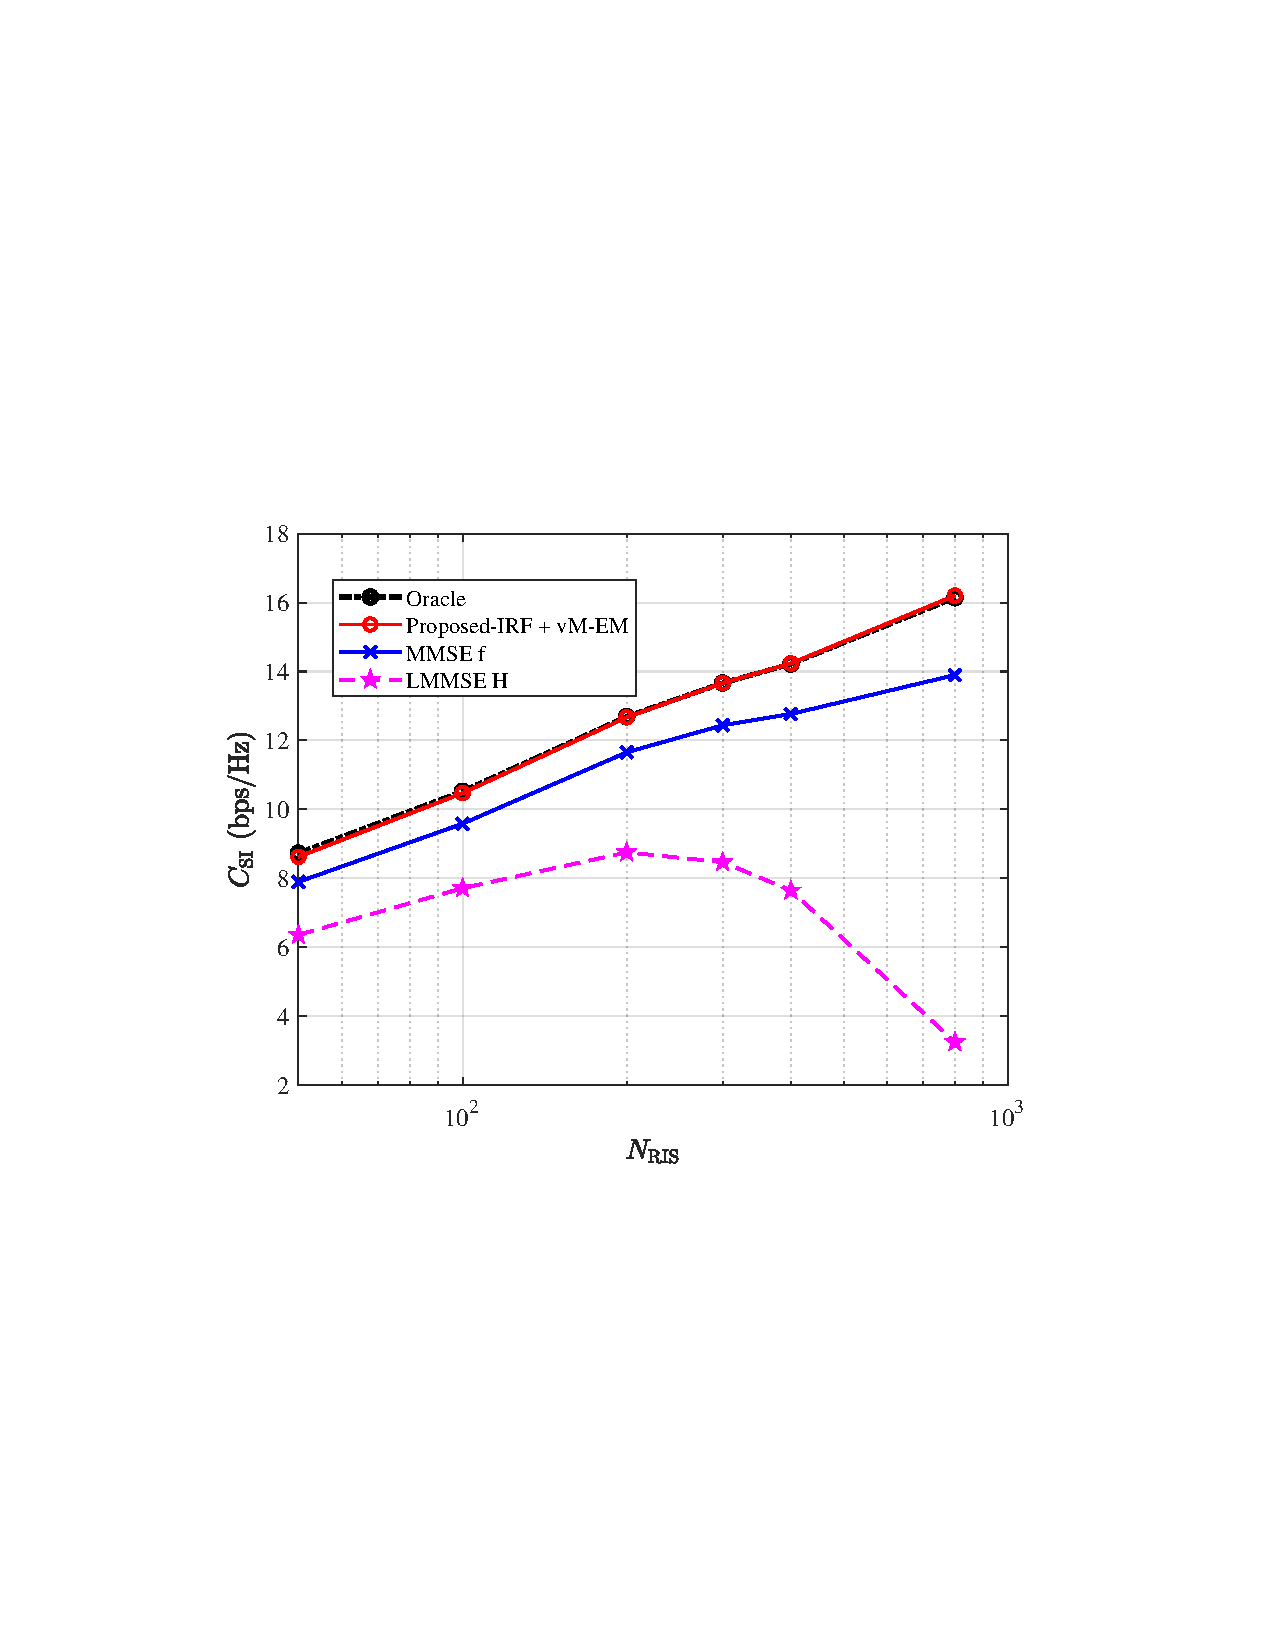
\includegraphics[width=0.7\textwidth]{figs/C-wrt-N_RIS.pdf}
    \caption{Comparison of the capacity upper bound $C_{\rm PSI}$ as a function of the RIS size $N$, where $M=8$. The definition of $C_{\rm PSI}$ will be explained in detail in response to question (6). }
    \label{fig:RIS_size}
\end{figure}

The simulation results are presented in {Fig.~\ref{fig:RIS_size}}. The black dashed Oracle line is obtained by assuming perfect knowledge about both the channel matrices $\bm G$ and $\bm f$; The red line represents the proposed IRF-based CSI acquisition scheme with known $\bm G$ and unknown $\bm f$; The MMSE-$\bm f$ baseline assumes the same channel knowledge as the proposed scheme, but calculates an MMSE estimation for $\bm f$ based on received uplink pilots at the BS; The LMMSE-$\bm H$ scheme assumes no prior channel knowledge. All these curves are drawn with respect to various RIS sizes $N$ ranging from $50$ to $800$. Note that the detailed values $N_y$ and $N_z$ of the planar RIS array are not important, since the i.i.d. Rayleigh fading channel is spatially unstructured.  

It can be derived from {Fig.~\ref{fig:RIS_size}} that, our proposed IRF-based scheme outperforms both of the MMSE schemes, and achieves near-optimal performance within a wide range of RIS sizes. The performance gain is mainly due to the reduced pilot overhead, since as the number of RIS element increases, the pilot overhead of the MMSE-based schemes scales linearly w.r.t. $N$, causing a proportional decrease in the average ergodic capacity per symbol $C_{\rm PSI}$. In the case $N\uparrow B=1000$ for LMMSE-$\bm H$ scheme, the capacity value even starts to drop significantly. However, the proposed IRF scheme does not subject to this capacity reduction, because the overhead is dimension-independent.  


3.3) The reviewer is concerned about the possible inefficiency of the proposed IRF-based RIS channel estimation method in the high sensor noise regime. It is true that if the sensor noise $\sigma_v^2$ is sufficiently large, then it is hard for the proposed IRF-based scheme to obtain any CSI knowledge. And usually, the low-cost power sensors are more noisy than the RF chain receivers. In order to penalize the accuracy of the cost-efficient sensors, we have manually injected more noise into the sensors by setting an additional sensor noise factor $F_p=10\,{\rm dB}$ and an enlarged sensor bandwidth $100\,{\rm MHz}$. The sensor noise is calculated according to 
\begin{equation*}
    \sigma_v^2 = F_p \times {\rm BW}_{\rm sensor}\, n_0,
\end{equation*}
where the thermal noise power spectral density is fixed to $n_0 =-174\,{\rm dBm/Hz}$. As a result, in our simulations, the sensor is set to be $F_p \times {\rm BW}_{\rm sensor}/{\rm BW}_{\rm RF} = 64.9\,{\rm dB}$ noisier than an RF-chain receiver. Even with this unfavorable situation, the IRF-based scheme still outperforms the traditional MMSE-based schemes, because of the {\it double-fading} effect [R6] of the reflective link will highly attenuates the reflective signal during traditional channel estimation. Note that the typical path loss at a distance of $100\,{\rm m}$ is $83.3\,{\rm dB}$ at $3.5\,{\rm GHz}$, and the {\it double-fading} effect doubles this number. 

[R6] M. Najafi, V. Jamali, R. Schober, and H. V. Poor, ``Physics-based modeling and scalable optimization of large intelligent reflecting surfaces,'' {\it IEEE Trans. Commun.}, vol. 69, no. 4, pp. 2673-2691, Apr. 2021.

}}


\textbf{Reviewer 1:}
4) It is not clear how BS beamforming vector $\bm w$ and user's scaler $w'$ are initialized in the proposed algorithms.

{\color{blue}{\textbf{Authors: } 
Thanks for pointing out this very important issue in our paper. We will try to answer this question in two parts. 

4.1) Scalers $\bm w$ and $w'$ during CSI acquisition. In our proposed IRF-based CSI acquisition algorithms, since the user's scaler $w'$ is introduced for the sake of symmetry with the BS's beamformer $\bm w$, it is always assumed that $w'\in\mathbb{R}_+$ equals the square root of the user's pilot transmit power, i.e., $w'$ is fixed to $\sqrt{P_{{\rm u}, p}}$, as is introduced in detail in~\eqref{eqn:transmit_power}. 
For our proposed IRF-based CSI acquisition algorithms, by assuming known BS-RIS link $\bm G$, a sub-optimal solution for $\bm w$ can be obtained by maximizing the total energy that the RIS receives during the creation of IRF, i.e., 
\begin{equation}
    {\bm w}_{\rm IRF} = \underset{\left\|{\bm w}\right\|\leq P_{{\rm BS}, p}}{\rm argmax}\left\|{\bm G}{\bm w} \right\|^2. 
    \label{eqn:IRF_w_opt}
\end{equation}
The solution to~\eqref{eqn:IRF_w_opt} is given by computing the singular value decomposition (SVD) ${\bm G} = {\bm U}{\bm S}{\bm V}\H$, sorting the diagonal entries of $\bm S$ in descending order, and setting ${\bm w}_{\rm IRF} = \sqrt{P_{{\rm BS}, p}}{\bm V}_{(:,1)}$, where ${\bm V}_{(:,1)}$ is the $1^{\rm st}$ column of the matrix ${\bm V}\in\mathbb{C}^{M\times M}$. 
Note that although the solution ${\bm w}_{\rm IRF}$ is a sub-optimal solution, it can still achieve nearly optimal spectral efficiency performance, which is demonstrated by our simulation results.  

4.2) Scalers $\bm w$ and $w'$ during downlink beamforming. For downlink transmission of a MISO system, the user's scaler $w'$ is dummy, so we only consider the BS's beamformer $\bm w$. In our proposed IRF-based method, after the CSI acquisition and the passive RIS beamforming, the BS's active beamformer is adjusted according to~\eqref{eqn:IRF_w_opt}. 
In contrast to this sub-optimal solution~\eqref{eqn:IRF_w_opt}, in the MMSE baselines, the BS's beamformer $\bm w$ is iteratively updated by exploiting the knowledge of the estimated channel $\hat{\bm H}$ according to the following two formulas
\begin{equation}
    \left\{\begin{aligned}
        & {\bm \theta}^{(t+1)} = \exp(-\ri \arg(\hat{\bm H}{\bm w}^{(t)})), \\
        & {\bm w}^{(t+1)} = {\rm norm}(\hat{\bm H}\H {\bm \theta}^{(t+1)*}),
    \end{aligned}\right.
\end{equation}
where ${\bm w}^{(0)}$ is randomly initialized such that $\|{\bm w}^{(0)}\| = \sqrt{P_{{\rm BS}, p}}$. Note that even if our proposed method employs a sub-optimal BS's beamformer $\bm w$, it still outperforms the baselines in terms of the achievable ergodic rate $C_{\rm PSI}$. 

In the revised paper, we have clarified the initialization and updating methods of the BS beamformer ${\bm w}$ and the user's scaler $w'$ for our proposed algorithms as well as the baselines, which is shown as follows.  
\begin{framed}\red{
    Moreover, for the IRF methods, the BS beamformer $\bm w$ is chosen to be the right singular vector that corresponds to the most significant singular value of the BS-RIS channel $\bm G$, which automatically maximizes the total signal energy received by the RIS from the BS, i.e., 
    \begin{equation*}
        {\bm w} = \underset{\left\|{\bm w}\right\|\leq P_{{\rm BS}, p}}{\rm argmax}\left\|{\bm G}{\bm w} \right\|^2,
    \end{equation*}
    and the user's transmit scaler is set to the maximum allowed power $w'=\sqrt{P_{{\rm u}, p}}$ for all the CSI acquisition schemes to ensure a high SNR. 
    For the LMMSE algorithms, after the channel estimation procedure, the beamforming step is fulfilled by alternately updating the BS beamformer $\bm w$ and the RIS phase-shift matrix $\bm\Theta = {\rm diag}({\bm \theta})$ according to  
    \begin{equation*}
        \left\{\begin{aligned}
            & {\bm \theta}^{(t+1)} = \exp(-\ri \arg(\hat{\bm H}{\bm w}^{(t)})), \\
            & {\bm w}^{(t+1)} = \sqrt{P_{{\rm BS}, d}}{\rm norm}(\hat{\bm H}\H {\bm \theta}^{(t+1)*}),
        \end{aligned}\right.
    \end{equation*}
    where ${\rm norm}({\bm z})$ denotes ${\bm z}/\left\|{\bm z}\right\|$. The initial values ${\bm w}^{(0)}$ and ${\bm\theta}^{(0)}$ are generated randomly, and both subject to their corresponding power constraint and unit-modulus constraint, respectively. In our simulations, the iteration is performed at most $T=10$ times. 
}
\end{framed}
}}



\textbf{Reviewer 1:}
5) It would be helpful to incorporate the number of time slots for channel estimation into {\bf Table I}.

{\color{blue}{\textbf{Authors: } 
Thanks for the suggestion of explicitly specifying the number of time slots for channel estimation in {\bf Table I}. In the revised paper, in order to clearly explain the pilot overhead of different schemes, we have changed the overhead index from ``Minimum pilot overhead'' to ``Minimum pilot overhead per user''. We have also clarified in the revised version that, the pilot overhead is equivalent to the number of time slots for channel estimation. Detailed revisions are shown as in the following box: 

\begin{framed}
\red{
    {\bf Table~1} compares the pilot overhead of our proposed IRF method with other different CSI acquisition methods. 
    All the CSI acquisition methods that appear in {\bf Table~1} assume a narrowband system, so the pilot overhead is equal to the number of pilot time slots.
    $K$ denotes the number of users, $S$ is the sparsity of the channel assumption, $M$ is the number of antennas at BS, and $\alpha$ is the ratio of the large-timescale channel  coherence time and the small-timescale channel coherence time [11]. 
    Except for CS-based methods [5], all the channel estimation methods [11], [13], [25] require the pilot overhead to be linearly dependent on $N$, while our IRF method needs a constant number of exactly 3 pilot slots per user, regardless of the number of RIS elements. 
}
\end{framed}
}}

\textbf{Reviewer 1:}
6) Fig.~8 $y$ axis is marked as capacity. However, it is understood that we only know the bound as in [R1]. It would be helpful to present the equations for capacity analysis.

[R1] A. Lapidoth and S. Shamai, ``Fading channels: how perfect need "perfect side information" be?,'' {\it IEEE Trans. Inf. Theory}, vol. 48, no. 5, pp. 1118-1134, May 2002. 

{\color{blue}{\textbf{Authors: } 
Many thanks to the reviewers for their comments on improving the strictness of this paper. In order to specify which capacity formula we employ in this paper, we first introduce the overall procedure of establishing a RIS-aided link. Specifically, we assume that the data transmission is preceded by three link establishment steps:
\begin{enumerate}
    \item Acquire the CSI (apply LMMSE or proposed IRF-based schemes), consuming $N_p$ time slots;
    \item Calculate BS's beamformer $\bm w$ and RIS's phase-shifts $\bm\Theta$ to maximize the user's received signal energy;
    \item Re-estimate the channel, assuming no additional pilot overhead.
\end{enumerate}
The step (3) is needed in real-world systems, because it is very possible that the equivalent BS-RIS-user channel ${\bm f}\H{\bm \Theta}{\bm G}{\bm w}\in\mathbb{C}$ changes significantly after the RIS reconfiguration and the BS beamforming. These changes are not perfectly predictable by previous CSI knowledge due to inaccurate RIS phase-shifts, phase-dependent reflective gain and imprecise BS beamforming. As a result, we assume that a perfect additional channel estimation step (3) is executed after the BS-RIS joint beamforming, and provides perfect CSI in the following data transmission. Since in this paper, we foucs on how to obtain CSI in step (1) for BS active beamforming and RIS passive beamforming in step (2), the pilot overhead for the re-estimation step (3) is omitted. This approximation is reasonable in that only one equivalent channel coefficient needs to be estimated in this step, which is much smaller compared to $NM$ coefficients involved in step (1). 

With this perfect CSI knowledge (side information) in step (3), we consider a block-fading channel with blocklength $B$. Within the same block, the random BS-RIS channel matrix $\bm G$ and the RIS-user channel vector ${\bm f}^*$ are realized for only once. After setting $\bm w$ and $\bm\Theta$ according to steps (1-2), the user's downlink SNR 
\begin{equation}
    \gamma_{\rm user} = \frac{P_{{\rm BS}, d} |{\bm f}\H {\bm \Theta} {\bm G}{\bm w}|^2}{\sigma_z^2}
\end{equation}
determines the ergodic channel capacity within the following $N_d = B-N_p$ data symbols. Thus, the ergodic capacity per channel use is given by 
\begin{equation}
    C_{\rm PSI} = \frac{N_d}{B} \mathbb{E}\left[\log\left( 1+\gamma_{\rm user} \right)\right], \label{eqn:capacity_def}
\end{equation} 
where the subscript PSI indicates that perfect side information [R1] is assumed after the establishment of the RIS-aided reflective link. In our simulations, the expectation in~\eqref{eqn:capacity_def} is numerically approximated by applying the Monte Carlo method. But rigorously speaking, the value $C_{\rm PSI}$ is an upper bound of the true channel capacity of the RIS-aided communication system. 


}}

{\color{blue}{\textbf{Authors: } 
Many thanks again for your valuable time and efforts to review this paper. 

Sincerely, \\
{\it The Authors }
}}

\begin{center}
    {\Large\bf Response to Reviewer 2's Comments}
\end{center}

\textbf{Reviewer 2:}
In this paper, the authors propose a dimension-independent channel state information (CSI) acquisition approach for reflecting intelligent surfaces (RIS) in which the required pilot overhead is independent of the number of RIS elements. The main idea is to estimate CSI based on received power variations when both the BS \& user simultaneously transmit to the RIS.

{\color{blue}{\textbf{Authors: } 
We appreciate the reviewer's concise summary of the key points of this paper. We have tried our best to revise the paper according to the reviewer's valuable comments, and our responses are provided in a point-to-point manner as below. 
}}

\textbf{Reviewer 2:}
While the proposed idea \& results seem correct, I do not believe the main contributions of the paper (largely algorithmic) are a good fit for IEEE Transactions on Information Theory. My recommendation to the authors would be to submit the paper to wireless communication- and/or signal processing-focused journals, which would be a better fit for the paper's contributions.

{\color{blue}{\textbf{Authors: } 
Much thanks for the reviewer's positive attitude on the novelty and correctness of this paper. Also, as is stressed by the reviewer, the previous version of this paper lacks a series of sound information-theoretic analyses. We agree with the reviewer that the analytical results are necessary for the high-quality journals like IEEE T-IT. To this end, we have tried our best to provide achievable bounds for our proposed interference random field (IRF)-based CSI acquisiton schemes. These newly-added theorems and lemmas are mainly related to detection and estimation theory, which may match the broader scope of this journal. For you to check, we have 

}}

%%%% Some strange ideas about the theory. 


\begin{theorem} 
    Suppose all the entries of ${\bm G}\in\mathbb{C}^{N\times M}$ and ${\bm f}\in\mathbb{C}^{N\times 1}$ obey ${\mathcal{CN}(0,1)}$ distribution, and the channel noise ${\bm N}\sim \mathcal{CN}(0,\sigma^2)$. 
    Then, the LS channel estimator is given by 
    \begin{equation}
        \hat{\bm{H}}_{\rm LS} = \left( {\bm F}_{N,P}^{*} {\bm F_{N,P}\T} \right)^{-1}{\bm F}_{N,P}^{*}{\bm Y}_{\rm BS}\T,
    \end{equation}
    and the MMSE estimator is given by 
    \begin{equation}
        \hat{\bm{H}}_{\rm MMSE} = \left( {\bm F}_{N,P}^{*} {\bm F_{N,P}\T + \sigma^2 {\bm I}_N} \right)^{-1}{\bm F}_{N,P}^{*}{\bm Y}_{\rm BS}\T
    \end{equation}
\end{theorem}

{\it Proof.}
Proof will be provided. 

The equivalent model can be expressed by 
\begin{equation}
    \tilde{\bm y}_{\rm BS} = {\rm vec}({\bm Y}_{\rm BS}) = {\bm A}{\bm h} + \tilde{\bm n},
\end{equation}
where ${\bm h} = {\rm vec}({\bm H}\T)\in\mathbb{C}^{NM}$, ${\bm A} = {\bm F}_{N,P}\T\otimes {\bm I}_M$, and $\tilde{\bm n} = {\rm vec}({\bm N})$. In this model, if we assume ${\bm C}_{\bm h} = $ 

\begin{theorem}
    With the MMSE channel estimator, the second-order statistics of the estimation error 
    \begin{equation}
        {\bm \epsilon} = {\rm vec}((\hat{{\bm H}}_{\rm MMSE} - {\bm H})\T)  
    \end{equation}
    is given by 
    \begin{equation}
        \mathbb{E}[{\bm \epsilon}{\bm \epsilon}\H | \hat{\bm h}] = \left( {\bm F}_{N,P}^{*} {\bm F_{N,P}\T / \sigma^2 + {\bm I}_N} \right)^{-1} \otimes {\bm I}_M.
    \end{equation}
\end{theorem}

Note that the distribution of such an estimation error ${\bm \epsilon}$ is not necessarily Gaussian. 



{\color{blue}{\textbf{Authors}}: We would like to commence by thanking the editor and three professional reviewers for their valuable time in evaluating our submission. Your constructive comments and expert knowledge of the field have helped us to strengthen the manuscript significantly. We endeavored to address all the suggestions and comments, and our reflections are provided below in a point-by-point way. We also indicate how our manuscript has been revised accordingly, and all the revisions have been highlighted in {\color{red} red} color in the revised paper. Here, we would like to make a brief summary of the major revisions in the revised paper as below:

1) We have clarified all the unclear statements pointed out by the reviewers, such as ``why the lens antenna array can realize the spatial DFT" and ``why we design the overall combining matrix ${{{\bf{\bar W}}}}$ as a Bernoulli random matrix".

2) We have justified all impractical assumptions pointed out by the reviewers, such as ``the number of path may not be known in advance" and ``the user may prefer the conventional antenna array instead of lens antenna array".

3) We have added the performance analysis of the proposed SSD-based scheme. It shows that this scheme can estimate the key parameters ${{\varphi _{l,c}}}$ for ${l = 1,2, \cdots ,L}$ with high probability.
}

\textbf{Editor}: As an editor, my major concern is the model (6), where ${{{\bf{W}}_q}}$ is known. Note that ${{{\bf{W}}_q}}$ is an ${{N_{{\rm{RF}}}} \times N}$ matrix combining the adaptive selecting network and RF chains,  and ${{{\bf{\tilde h}}_m}}$ is majorly the propagation channel. Typically, in wireless communication, RF impairments are captured in the baseband channel, and the propagation channel + RF chain gain/phase are the estimated baseband channel. But, in the assumed model, ${{{\bf{W}}_q}}$ is an ${{N_{{\rm{RF}}}} \times N}$ matrix and has ${{N_{{\rm{RF}}}} \times N}$ elements. We may assume that ${{{\bf{W}}_q}}$ is known using a nominal value, but in this case the unknown impairment or gain/phase offset in ${{{\bf{W}}_q}}$ (from the known nominal ${{{\bf{W}}_q}}$) should be able to be captured in ${{{\bf{\tilde h}}_m}}$. But, ${{{\bf{\tilde h}}_m}}$ is a column vector, so the unknown impairment or gain/phase offset in ${{{\bf{W}}_q}}$ should be identical for each column. I am not sure about this. If so, please explain this in the revision.  If the unknown impairment is elementwise in ${{{\bf{W}}_q}}$, then the model (6) is not valid.

{\color{blue} \textbf{Authors}: Thanks for pointing out this important issue. Actually, the RF impairments of ${{{\bf{W}}_q}}$ include two parts. The first one is the impairment incurred by the RF chains. This impairment should be identical for each row of ${{{\bf{W}}_q}}$, and therefore can be captured in the estimated channel as pointed out by the Editor. The second one is the impairment incurred by the phase shifters in the adaptive selecting network. This impairment is element-wise, and it cannot be fully captured in the estimated channel. We would like to point out that this problem commonly exists in most of the channel estimation schemes for hybrid analog and digital architecture, since the analog module (e.g., phase shifter network or lens) is usually involved in the channel estimation procedure [R1].



Fortunately, when hardware impairment incurred by the analog module is not serious (this is reasonable since only the analog module working stably will be used), it will not result in significant accuracy degradation in channel estimation. This conclusion can be verified by the following Fig. 1, where the parameters are the same as those for Fig. 10 in the paper. In Fig. 1, the dash lines present the case without hardware impairment, i.e., ${{{\bf{W}}_{q,{\rm{real}}}} = {{\bf{W}}_q}}$, while the solid lines present the case with hardware impairment incurred by the phase shifters in the adaptive selecting network, i.e., ${{{\bf{W}}_{q,{\rm{real}}}} = {\bf{E}} \odot {{\bf{W}}_q}}$, where ${ \odot }$ denotes the element-wise multiplication, ${{\bf{E}}}$ is an ${{N_{{\rm{RF}}}} \times N}$ impairment matrix. Note that each element ${{e_{ij}}}$ of ${{\bf{E}}}$ is modeled as ${{e_{ij}} = \left| {{e_{ij}}} \right|\exp \left( {j{\phi _{ij}}} \right)}$, where ${\left| {{e_{ij}}} \right|\sim{\cal U}\left( {0.9,1.1} \right)}$ presents the gain with offset, ${{\phi _{ij}} \sim {\cal U}\left( { - {{10}^ \circ },{{10}^ \circ }} \right)}$ presents the phase with offset, and ${{\cal U}\left( {a,b} \right)}$ denotes the uniform distribution between ${a}$ and ${b}$ [R1]. Fig. 1 shows that the accuracy degradation caused by the hardware impairment is not significant, and the proposed SSD-based scheme can still achieve the satisfying accuracy close to the ideal oracle LS scheme.

Fig. 1. Impact of hardware impairment on the proposed SSD-based scheme.

In the revised paper, we have addressed this issue as:
\begin{framed}
{\color{red} Finally, it should be noted that the hardware impairment may exist in the adaptive selecting network, leading to the element-wise gain/phase offset in ${{{\bf{W}}_q}}$, which cannot be fully captured in the estimated channel. This is a common problem existing in most of channel estimation schemes for hybrid analog and digital architecture [4], since the analog module (e.g., phase shifter network) is usually involved in the channel estimation procedure. Fortunately, since the gain/phase offsets are usually not serious in practice, the accuracy degradation in channel estimation caused by this hardware impairment will not be significant.}
\end{framed}

[R1] R. W. Heath, N. Gonzalez-Prelcic, S. Rangan, W. Roh, and A. Sayeed, ``An overview of signal processing techniques for millimeter wave MIMO systems," {\it IEEE J. Sel. Top. Signal Process.}, vol. 10, no. 3, pp. 436-453, Apr. 2016.



\vbox{}

{\color{blue} \textbf{Authors}: Many thanks again for your valuable time and efforts to review this paper.
\\
\\
Sincerely,

 {\it The Authors}}


}




\clearpage
\begin{center}
 {\Large\bf Response to Reviewer 1's Comments}
\end{center}


\textbf{Reviewer 1}: The paper proposes an efficient technique for the wideband beamspace channel estimation problem for mmWave using lens antenna arrays. By exploiting similar beam directions across antennas for a given path, the proposed technique can estimate mmWave channels using lens antennas without assuming a common support set across frequency bands. The proposed technique seems to be novel, and the paper is well written. I have some comments before its publication.


{\color{blue} \textbf{Authors}: We appreciate the reviewer's concise summary of the key points of this paper and the positive evaluation on our work. We have tried our best to revise the paper according to the reviewer's valuable comments, and our responses are provided in the point-by-point way as below.}

\textbf{Reviewer 1}: 1) It is not clear at first why, for a given path, the support sets of different antennas are similar as in (9). I think this can be intuitively explained using a figure with antennas and beams, i.e., with far field assumption in microwave, the beam direction is the same for all antennas, with extremely small wavelength of mmWave; however, the beam direction would be different, but similar, across antennas. This conceptual explanation would help understanding the core idea of paper.

{\color{blue} \textbf{Authors}: Thanks for the suggestion of clearly explaining why the support of each path component has the similar beam indices as in Eq. (9). To answer this question, we first provide the definition of each path component in the beamspace as below:
$$
{{\bf{\tilde c}}_{l,m}} = {\bf{U}}_a^H{\bf{a}}\left( {{\varphi _{l,m}}} \right) = {\left[ {\Xi \left( {{\varphi _{l,m}} - {{\bar \varphi }_1}} \right),\Xi \left( {{\varphi _{l,m}} - {{\bar \varphi }_2}} \right), \cdots ,\Xi \left( {{\varphi _{l,m}} - {{\bar \varphi }_N}} \right)} \right]^T},
$$
where ${\Xi \left( x \right) = \frac{{\sin N\pi x}}{{\sin \pi x}}}$ is the Dirichlet sinc function as shown in the following Fig. 1. Ideally, when the ${{{\varphi _{l,m}}}}$ is exactly the same as one of the beam directions ${{\bar \varphi _1},{\bar \varphi _2}, \cdots {\bar \varphi _N}}$ pre-defined by lens antenna array, the power of ${{{\bf{\tilde c}}_{l,m}}}$ will be focused on only one beam, as shown by the red dash lines in Fig. 1. However, in practice, ${{{\varphi _{l,m}}}}$ is arbitrary, which may be different from the pre-defined beam directions. In this case, the path power will be distributed on several pre-defined beams. According to the property of ${\Xi \left( x \right)}$, i.e., ${\Xi \left( x \right)}$ is larger when ${x}$ is closer to 0, we know that the indices of these power-focused beams should be adjacent (similar) as shown by the blue dot dash lines in Fig. 1. More detailed proof can be found in [R1, Lemma 2].



In the revised paper, we have explained Eq. (9) more clearly as:
\begin{framed}
{\color{red} The reasonability of (9) can be explained as follows. In practice, ${{{\varphi _{l,m}}}}$ is arbitrary, which is usually different from the pre-defined beam directions ${{\bar \varphi _1},{\bar \varphi _2}, \cdots {\bar \varphi _N}}$. In this case, the power of ${{{\bf{\tilde c}}_{l,m}}}$ will be distributed on several beams. According to the property of ${\Xi \left( x \right)}$ in ${{{\bf{\tilde c}}_{l,m}}}$, i.e., ${\Xi \left( x \right)}$ is larger when ${x}$ is closer to 0, we know that the indices of these power-focused beams should be adjacent. More detailed proof can be found in [18, Lemma 2].}
\end{framed}


\vspace*{-10mm}
Fig. 1. The normalized power distribution of ${{\bf{\tilde c}}_{l,m}}$.

[R1] X. Gao, L. Dai, S. Han, C.-L. I, and X. Wang, ``Reliable beamspace channel estimation for millimeter-wave massive MIMO systems with lens antenna array," {\it IEEE Trans. Wireless Commun.}, vol. 16, no. 9, pp. 6010-6021, Sep. 2017.
}

\textbf{Reviewer 1}: 2) The paper assumes that the receiver combining matrix ${{\bf{\bar W}}}$ consists of -1 or +1 with proper normalization. Is this a necessary condition for the proposed technique? If yes, please explicitly mention this in the paper. If not, I think it would be better to generalize the combining matrix.


{\color{blue} \textbf{Authors}: Thanks for this important comment. The receiver combining matrix ${{\bf{\bar W}}}$ with normalized elements of -1 or 1  (i.e., ${{\bf{\bar W}}}$ is a Bernoulli random matrix) is not a necessary condition for the proposed technique. We use the Bernoulli random matrix due to the following two reasons: i) it can be easily realized by the 1-bit phase shifters with low hardware cost and energy consumption [R1]; ii) it enjoys low mutual-column coherence, and therefore can be expected to achieve high recovery accuracy according to the compressive sensing theory [R2].

However, if ${{\bf{\bar W}}}$ is not a Bernoulli random matrix, our scheme can still work. One example is shown in the following Fig. 2. Here, we design ${{\bf{\bar W}}}$ as a matrix, whose elements have the same normalized amplitude ${\frac{1}{{\sqrt {Q{N_{{\rm{RF}}}}} }}}$ but with arbitrary phases (realized by the high-resolution phase shifters). The other parameters for Fig. 2 are the same as those for Fig. 10 in the paper. It shows that our scheme can still achieve higher accuracy than the conventional schemes.


Fig. 2. NMSE comparison against the SNR for channel estimation when the elements of ${{\bf{\bar W}}}$ have the same normalized amplitude but with arbitrary phases.

To address this comment, in the revised paper, we have modified the description of ${{\bf{\bar W}}}$ as:
\begin{framed}
{\color{red} Furthermore, we define
${{\bf{\bar W}} = \left[{{\bf{W}}_1^T,{\bf{W}}_2^T, \cdots ,{\bf{W}}_Q^T} \right]^T}$ of size ${Q{N_{{\rm{RF}}}} \times N}$ as the overall combing matrix, which is designed according to the hardware realization of the adaptive selecting network. For example, if the adaptive selecting network is realized by the low-cost 1-bit phase shifters as in [18], the elements of ${{\bf{\bar W}}}$ can be randomly selected from the set ${\frac{1}{\sqrt{Q{{N}_{\text{RF}}}}}\left\{ -1,+1 \right\}}$ with equal probability.}
\end{framed}

[R2] D. L. Donoho, ``Compressed sensing," {\it IEEE Trans. Inf. Theory}, vol. 52, no. 4, pp. 1289-1306, Apr. 2006.

}

\textbf{Reviewer 1}: 3) In the first term (inside the integral) in the last line of (20), isn't ${- \Delta \varphi}$ correct?


{\color{blue} \textbf{Authors}: Thanks for the reviewer's careful check. The first term in the last line of Eq. (20) should be ${\int_{ - \frac{{{\alpha _n}}}{2}}^{\frac{{{\alpha _n}}}{2}} {{\Xi ^2}\left( {\frac{{{\Delta _n}}}{N} - \Delta \varphi } \right)d\Delta \varphi }}$. However, it can be also equivalently expressed as ${\int_{ - \frac{{{\alpha _n}}}{2}}^{\frac{{{\alpha _n}}}{2}} {{\Xi ^2}\left( {\frac{{{\Delta _n}}}{N} + \Delta \varphi } \right)d\Delta \varphi }}$ as shown in the previous paper. This can be explained as follows:
\begin{align}\label{eq1}
\nonumber \int_{ - \frac{{{\alpha _n}}}{2}}^{\frac{{{\alpha _n}}}{2}} {{\Xi ^2}\left( {\frac{{{\Delta _n}}}{N} - \Delta \varphi } \right)d\Delta \varphi } &\mathop  = \limits^{\left( a \right)} \int_{\frac{{{\alpha _n}}}{2}}^{ - \frac{{{\alpha _n}}}{2}} {{\Xi ^2}\left( {\frac{{{\Delta _n}}}{N} + x} \right)d\left( { - x} \right)} \\ \nonumber
& = \int_{ - \frac{{{\alpha _n}}}{2}}^{\frac{{{\alpha _n}}}{2}} {{\Xi ^2}\left( {\frac{{{\Delta _n}}}{N} + x} \right)dx} = \int_{ - \frac{{{\alpha _n}}}{2}}^{\frac{{{\alpha _n}}}{2}} {{\Xi ^2}\left( {\frac{{{\Delta _n}}}{N} + \Delta \varphi } \right)d\Delta \varphi },
\end{align}
where ${\left( a \right)}$ is obtained by letting ${x =  - \Delta \varphi}$.

}


\textbf{Reviewer 1}: 4) In Fig. 5, it would be better to have some intuitive explanations why ${{\Delta _n}}$ varies with ${n}$.

{\color{blue} \textbf{Authors}: Thanks for this suggestion. In the revised paper, we have explained why ${{\Delta _n}}$ varies with ${n}$ as:
\begin{framed}
{\color{red} Moreover, Fig. 5 also shows that the derived ${{\Delta _n}}$ varies when ${{\varphi _{l,c}}}$ equals different ${{\bar \varphi _n}}$ (leading to different ${{{\bf{C}}_n}}$ defined in \textbf{Lemma 2}). The reason is that different ${{\varphi _{l,c}}}$ incur different degrees of power leakage due to beam squit. Therefore, we need to change ${{\Delta _n}}$ to make sure that we can always capture most of the power of ${{{\bf{C}}_n}}$.}
\end{framed}

}

\textbf{Reviewer 1}: 5) In the simulation section, please define NMSE mathematically.

{\color{blue} \textbf{Authors}: Thanks for this suggestion. In the revised paper, we have added the mathematical definition of NMSE in Section V (Simulation Results) as:
\begin{framed}
{\color{red} Finally, we use the normalized mean square error (NMSE) to measure the accuracy of channel estimation for each user, which is mathematically defined as

$$
\mathbb{E}\left( {\frac{1}{M}\sum\limits_{m = 1}^M {\frac{{\left\| {{{{\bf{\tilde h}}}_m} - {\bf{\tilde h}}_m^e} \right\|_2^2}}{{\left\| {{{{\bf{\tilde h}}}_m}} \right\|_2^2}}} } \right), \eqno(77)
$$
where ${{{\bf{\tilde h}}_m^e}}$ is the estimated beamspace channel at sub-carrier ${m}$.}
\end{framed}
}



\textbf{Reviewer 1}: 6) The authors explained why there exists an error floor at high SNR in Fig. 9. It is not clear with this explanation why ``Oracle LS scheme" also experiences such a floor. Please elaborate this.


{\color{blue} \textbf{Authors}: Thanks for this insightful comment. Actually, in the oracle LS scheme, we also regard the elements of beamspace channel with very low power as zeros, as we have done in all the considered schemes. The only difference is that the positions of the elements with large power are assumed to be perfectly known in the oracle LS scheme, and that is why the word ``oracle" is used. Therefore, even for the oracle LS scheme, it still experiences a NMSE floor at high SNR. In the revised paper, we have explained this issue more clearly as:

\begin{framed}
{\color{red} Note that for all the schemes mentioned above, we regard the elements of wideband beamspace channel with indices outside the support as zeros.}
\end{framed}
}

\textbf{Reviewer 1}: 7) In Fig. 11, why is the performance order of SOMP and OMP different with channel estimation SNRs?

{\color{blue} \textbf{Authors}: Thanks for pointing out this important issue. When the SNR for data transmission is low, the sum-rate performance of wideband beam selection is dominated by noise. In this case, all the schemes enjoy the same performance order even if the SNR for channel estimation is changed. However, when the SNR for data transmission is high, the sum-rate performance is dominated by channel estimation error. Therefore, different SNRs for channel estimation will lead to different performance order. In the revised paper, we have addressed this issues as: 
\begin{framed}
{\color{red} Finally, we observe that the performance orders of all schemes change with the SNR for channel estimation. This is due to the fact that when the SNR for data transmission is high, the sum-rate performance of wideband beam selection is dominated by channel estimation error.}
\end{framed}
}

\textbf{Reviewer 1}: 8). In Fig. 13, the SNR for channel estimation should be quite high, the value that might be impractical, even for ``Oracle LS scheme". With this result, it seems a bit pessimistic to have accurate CSI with multiple antennas at UEs. Is there any way to improve this?

{\color{blue} \textbf{Authors}: Thanks for this insightful comment. It is true that the required SNR for channel estimation  is quite high in the case with multiple-antenna users. This is because that the dimension of beamspace channel is significantly increased, and the number of nonzero elements to be estimated is much lager than the number in the case with single-antenna users. This problem can be partly solved by increasing the pilot overhead. Moreover, as we can see from Fig. 11 in the previous paper (Fig. 12 in the revised paper), even if the SNR for channel estimation is not high enough (e.g., 0 dB or 15 dB), wideband beam selection can still achieve satisfying sum-rate. This is due to the fact that for data transmission, only the  reduced-dimensional beamspace channel with much smaller size is effective. Therefore, when the SNR for channel estimation is not high enough, although the total NMSE performance is not satisfying, the reduced-dimensional beamspace channel may already be accurate. This means that we do not need to estimate the beamspace channel so accurately at the cost of high SNR in practice.


Fig. 11. (Fig. 12 in the revised paper) Sum-rate comparison against the SNR for data transmission.


In the revised paper, we have addressed this issue as:
\begin{framed}
{\color{red} Moreover, we would like to point out that in the case with multiple-antenna users, the required SNR for channel estimation to achieve satisfying NMSE is usually larger than the case with single-antenna users. However, as we can see from Fig. 12, even if the SNR for channel estimation is not high enough (e.g., 0 dB or 15 dB), wideband beam selection can still achieve satisfying sum-rate. The reason is that for data transmission, only the  reduced-dimensional beamspace channel with much smaller size is effective. Although the  NMSE performance may not be good enough with low SNR for channel estimation, the  reduced-dimensional beamspace channel is already accurate enough for data transmission. Therefore, in practice we do not need to estimate the beamspace channel so accurately at the cost of high SNR.}
\end{framed}



}

\vbox{}

{\color{blue} \textbf{Authors}: Many thanks again for your valuable time and efforts to review this paper.
\\
\\
Sincerely,

 {\it The Authors}}


\clearpage
\begin{center}
 {\Large\bf Response to Reviewer 2's Comments}
\end{center}

\textbf{Reviewer 2}: In this paper, the authors study a millimeter wave lens antenna array system. In particular, the authors focus on the beamspace channel estimation in wideband communication. It firstly shows that the antenna support of the beamspace channel depends on the frequency, and then proposes a successive support detection based scheme for channel estimation. The paper is well written in general. The studied topic is interesting and timely. The contribution is solid. I have the following comments.


{\color{blue} \textbf{Authors}: We appreciate the reviewer's concise summary of the key contributions of our paper and the positive evaluation on our work as well. To address your professional comments, we have made several major revisions in the revised paper, which are described one by one as below.
}

\textbf{Reviewer 2}: 1) It is unclear what is the fundamental principle of lens antenna array so as to achieve the spatial discrete fourier transform (DFT). In particular,  for wideband channels, is the response of the lens antenna array also frequency-dependent, such as the expression given in (1)?

{\color{blue} \textbf{Authors}: Thanks for this insightful comment. The reason why lens antenna array realizes the function of spatial DFT has been analyzed in [R1, Lemma 1]. Briefly, the electromagnetic lens is similar to the optical lens, which is able to change the propagation directions of the electromagnetic rays to achieve the energy focusing or beam collimation capability. As shown in the following Fig. 1, this means that all the plane electromagnetic rays with a incidence ${\phi }$ should arrive at one feed antenna ${B}$ located on the lens focal surface with identical phase for constructive superposition. To achieve this target, we need to design the phase shift profile ${\Phi \left( {y,z} \right)}$, which is realized by the spatial phase shifter at any point ${\left( {0,y,z} \right)}$ on the lens's aperture. With some mathematical derivations, it can be finally shown that based on the carefully designed phase shift profile, the electromagnetic rays received at the lens focal surface can be well-approximated as the spatial DFT of the ones received at the lens's aperture.

Next, we will explain whether the response of the lens antenna array is frequency-dependent. As we have mentioned above, realizing the power-focusing capability of lens requires us to carefully design the phase shift profile ${\Phi \left( {y,z} \right)}$ of the spatial phase shifters on the lens's aperture. In general, the spatial phase shifters can be realized by different analog modules, such as a class of bandpass surfaces or even the conventional phase shifters [R2]. However, most of this analog modules can not be  adjusted according to different frequencies [R3]. As a result, when the electromagnetic rays with different frequencies arrive at the lens aperture, they will be focused on different feed antennas, which means that the response of lens antenna array can not be frequency-dependent as the expression given in Eq. (1) in the paper.



Fig. 1. A planar lens placed in the y-z plane with the feed antennas located on its focal surface.

Finally, we would like to admit that it is possible but challenging that a frequency-dependent lens antenna array compensating for the effect of beam squint can be manufactured. In this case, our proposed SSD-based scheme can be further simplified to the narrowband version, since we do not need to generate several beamspace windows to estimate the spatial direction of each path at the carrier frequency any more.

In the revised paper, we have addressed this issues as:
\begin{framed}
{\color{red} The reason why lens antenna array realizes the spatial DFT can be found in [10, \textbf{Lemma 1}]. It shows that the power-focusing capability of lens relies on the spatial phase shifters on lens's aperture, which usually cannot be adjusted according to different frequencies. As a result, the response of lens antenna array cannot be frequency-dependent as in (1). However, we would like to admit that it is possible but challenging that a frequency-dependent lens antenna array compensating for the effect of beam squint can be manufactured. In this case, the proposed SSD-based scheme can be further simplified to the narrowband version as we have proposed in [18], since the OFDM is adopted.}
\end{framed}


[R1] Y. Zeng and R. Zhang, ``Millimeter wave MIMO with lens antenna array: A new path division multiplexing paradigm," {\it IEEE Trans. Commun.}, vol. 64, no. 4, pp. 1557-1571, Apr. 2016.

[R2] M. A. Al-Joumayly and N. Behdad, ``Wideband planar microwave lenses using sub-wavelength spatial phase shifters," {\it IEEE Trans. Antennas Propag.}, vol. 59, no. 12, pp. 4542-4552, Dec. 2011.

[R3] R. W. Heath, N. Gonzalez-Prelcic, S. Rangan, W. Roh, and A. Sayeed, ``An overview of signal processing techniques for millimeter wave MIMO systems," {\it IEEE J. Sel. Top. Signal Process.}, vol. 10, no. 3, pp. 436-453, Apr. 2016.


Fig. 3. (in the revised paper) Beam power variation over frequency.

}

\textbf{Reviewer 2}: 2) How is Fig. 3 related to the definition of the beamspace ${{{\bf{\tilde c}}_{l,m}}}$ given in (5)? It seems that (5) is given only in the discrete frequencies at each sub-carrier ${m}$, whereas Fig. 3 is in continuous frequency. Besides, what does the index ${n}$ represent?

{\color{blue} \textbf{Authors}: Thanks for pointing out this important issue. In this revised paper, we have modified Fig. 3 to the discrete frequencies case (also provided as below) to make it consistent with Eq. (5). Moreover, we have also explained what is the index ${n}$ as:


\begin{framed}
{\color{red} Fig. 3 shows the effect of beam squint from another perspective, where the parameters are the same as Fig. 2, and the curve indexed by ${n}$ represents the power variation of the ${n}$th element (beam) of ${{{\bf{\tilde c}}_{l,m}}}$  over frequency.}
\end{framed}




}

\textbf{Reviewer 2}: 3) In Fig. 1, an adaptive selecting network is shown after the lens antenna array, whereas below equation (7), a combiner matrix with 1-bit phase shifters is used. This seems to be inconsistent as we would simply expect antenna selection based on Fig. 1.

{\color{blue} \textbf{Authors}: Thanks for this comment. In this paper, we utilize 1-bit phase shifters instead of the conventional switches to realize the adaptive selecting work as in [R4] due to the following two facts: i) 1-bit phase shifters also have low cost as the conventional switches. Therefore, the additional hardware cost and energy consumption incurred by 1-bit phase shifters are not significant [R4]; ii) the correspondingly designed ${{\bf{\bar W}}}$ has been proved to enjoy low mutual-column coherence. Therefore, it can be expected to achieve high recovery accuracy according to the compressive sensing theory [R5].

Fig. 2. Typical architecture of phase shifter [R6].

However, we would like to point out that even if the adaptive selecting network is realized by 1-bit phase shifters, it can still be configured to realize the traditional function of beam selection during the data transmission. Specifically, we can turn off some phase shifters to realize ``unselect" and set some phase shifters to shift the phase 0 degree to realize ``select" in beam selection. Next, we will explain how to turn off the phase shifters in practice. The typical architecture of phase shifter is shown in Fig. 2 as below, where the phase shifts are quantified and controlled by digital signals [R6]. Fig. 2 shows that the phase shifter can be considered as the combination between switches and transmission lines with different lengths. Therefore, when the phase shifter should be turned off, we can just turn off the corresponding switches.



In the revised paper, we have addressed this issue as:
\begin{framed}
{\color{red} It is worth pointing out that during the data transmission, such adaptive selecting network with 1-bit phase shifters can also be configured to realize the conventional beam selection [12]. To do this, we can turn off some phase shifters to realize ``unselect" [32] and set some phase shifters to shift the phase 0 degree to realize ``select".}
\end{framed}


[R4] X. Gao, L. Dai, S. Han, C.-L. I, and X. Wang, ``Reliable beamspace channel estimation for millimeter-wave massive MIMO systems with lens antenna array," {\it IEEE Trans. Wireless Commun.}, vol. 16, no. 9, pp. 6010-6021, Sep. 2017.

[R5] D. L. Donoho, ``Compressed sensing," {\it IEEE Trans. Inf. Theory}, vol. 52, no. 4, pp. 1289-1306, Apr. 2006.

[R6] N. Tucker, ``A low cost electro-mechanical phase shifter design, including a brief summary of solid state methods," available at www.activefrance.com.

}

\textbf{Reviewer 2}: 4) Furthermore, the authors are advised to explain why a randomly selected combining matrix ${{\bf{\bar W}}}$ is a good choice.

{\color{blue} \textbf{Authors}: Thanks for this suggestion. In the revised paper, we have explained why we design ${{\bf{\bar W}}}$ as a randomly selected matrix by:
\begin{framed}
{\color{red} The reason we adopt the randomly selected matrix is that it has been proved to enjoy low mutual-column coherence, and therefore can be expected to achieve high recovery accuracy according to the compressive sensing theory [34].}
\end{framed}

}

\textbf{Reviewer 2}: 5) For the proposed SSD-based channel estimation scheme, is there any requirement on a prior knowledge of the channel, such as the total number of the resolvable paths ${L}$?

{\color{blue} \textbf{Authors}: Yes, for the proposed SSD-based scheme, we assume that the number of resolvable paths ${L}$ is known. This is due to the fact that a suggested ${L}$ can be usually obtained by channel measurement in advance. For example, a measurement report in New York City has shown that the average number of resolvable paths in 28 GHz propagation environment is 6.8 with a standard deviation of 2.2 [R7]. Therefore, for the specific environment, ${L}$ can be directly set as the largest possible value (e.g., in New York City, we set ${L = 6.8+2.2 = 9}$). In practice, the actual number ${L_a}$ of resolvable paths should be a little smaller than ${L}$, but this will not significantly affect the performance of the proposed SSD-based scheme. One example is shown in the following Fig. 3, where the parameters are the same as those for Fig. 10 in the paper except that ${L \ge L_a = 3}$. We observe that even if ${L}$ is a little larger than ${L_a}$, our scheme still enjoys satisfying accuracy.

Fig. 3. NMSE comparison against the assumed number of resolvable paths ${L}$.

Moreover, we would like to point out that the prior knowledge of ${L}$ is not the necessary condition in the proposed SSD-based scheme. When ${L}$ cannot be obtained in advance, we can borrow the idea of the classical OMP and SOMP algorithms, and run the proposed SSD-based scheme for several times [R8]. Specifically, during the ${t}$-th running (${t = 1,2, \cdots }$), we set ${L = t}$, and define the channel estimation update as ${\frac{1}{{MN}}\left\| {{{{\bf{\tilde H}}}^{\left( t \right)}} - {{{\bf{\tilde H}}}^{\left( {t - 1} \right)}}} \right\|_F^2}$, where ${{{{{\bf{\tilde H}}}^{\left( {t - 1} \right)}}}}$ and ${{{{{\bf{\tilde H}}}^{\left( t \right)}}}}$ are the previous estimated channel at the ${\left( {t - 1} \right)}$-th running and the current estimated channel at the ${t}$-th running, respectively. If the update is smaller than a threshold ${\zeta }$, then we will terminate. The following Fig. 4 shows the NMSE comparison between the SSD-based scheme with known ${L}$ and the one with unknown ${L}$, where we empirically set ${\zeta = 0.1}$. We observe that by utilizing this method, we can obtain the solution quite close to the one when ${L}$ is known in advance.


Fig. 4. (Fig. 10 in the revised paper) NMSE comparison between the SSD-based scheme with known and unknown ${L}$.



In the revised paper, we have addressed this issue as:
\begin{framed}
{\color{red} Actually, a suggested ${L}$ can be usually obtained in advance by channel measurement [24]. For example, a measurement report in New York City has shown that the average number of resolvable paths in 28 GHz propagation environment is 6.8 with a standard deviation of 2.2, and therefore we can set ${L}$ as the largest possible value as ${L = 9}$ in this case. In practice, the actual number of resolvable paths should be a little smaller than ${L}$, but this will not significantly affect the performance of the proposed SSD-based scheme. Moreover, it is worth pointing out that the prior knowledge of ${L}$ is not a necessary condition in our scheme. When ${L}$ cannot be obtained in advance, we can borrow the idea of the classical OMP and SOMP algorithms, and run the proposed SSD-based scheme for several times [35]. Specifically, during the ${t}$-th running (${t = 1,2, \cdots }$), we set ${L = t}$, and define the channel estimation update as ${\frac{1}{{MN}}\left\| {{{{\bf{\tilde H}}}^{\left( t \right)}} - {{{\bf{\tilde H}}}^{\left( {t - 1} \right)}}} \right\|_F^2}$, where ${{{{{\bf{\tilde H}}}^{\left( {t - 1} \right)}}}}$ and ${{{{{\bf{\tilde H}}}^{\left( t \right)}}}}$ are the previous estimated channel at the ${\left( {t - 1} \right)}$-th running and the current estimated channel at the ${t}$-th running, respectively. If the update is smaller than a threshold ${\zeta }$ (e.g., ${\zeta = 0.1}$), then we will terminate. In Section V, we will verify that by utilizing this method, the proposed SSD-based scheme can still achieve satisfying accuracy without the knowledge of ${L}$.}
\end{framed}




[R7] T. S. Rappaport, S. Sun, R. Mayzus, H. Zhao, Y. Azar, K. Wang, G. N. Wong, J. K. Schulz, M. Samimi, and F. Gutierrez, ``Millimeter wave mobile communications for 5G cellular: It will work!" {\it IEEE Access}, vol. 1, pp. 335-349, May 2013.

[R8] M. F. Duarte and Y. C. Eldar, ``Structured compressed sensing: From theory to applications," {\it IEEE Trans. Signal Process.}, vol. 59, no. 9, pp. 4053-4085, Sep. 2011.

}

\textbf{Reviewer 2}: 6) In Section IV, the users are assumed to employ also lens antenna array. However, lens antenna array is usually bulky compared to conventional array. Is it feasible to be employed at the user side? Another possibility is for the user to employ a small conventional antenna array. Is the proposed scheme applicable to such setup as well?


{\color{blue} \textbf{Authors}: Thanks for pointing out this important issue. The reviewer is right that in practice the users are more likely to employ the conventional antenna array, since currently the lens antenna array is usually bulky. However, we would like to point out that the proposed SSD-based scheme can also work when the users employ the conventional antenna arrays. In this case, the power of wideband beamspace channel at one sub-carrier is focused on a small number of rows instead of a small number of low-dimensional sub-matrices. One example is shown in the following Fig. 5, where we set the number of BS antennas ${N = 64}$ and the number of user antennas ${U = 16}$. This property enables us to further simplify our scheme described in Section IV (Extension to Multiple-Antenna Users). Specifically, when the conventional antenna array is employed at the user side, we do not need to estimate the column support ${{{{\cal S}_{l,m}}}}$ of each path component any more. After we have estimated the row support ${{{{\cal T}_{l,m}}}}$ by Eq. (72) and Eq. (74) in the paper, the support of the ${l}$-th path component can be directly obtained as ${{{\cal D}_{l,m}} = \left\{ {n + \left( {u - 1} \right)N\left| {n \in {{\cal T}_{l,m}},u \in \left\{ {1,2, \cdots ,U} \right\}} \right.} \right\}}$ instead of ${{\cal D}_{l,m}} = \left\{ {n + \left( {u - 1} \right)N\left| {n \in {{\cal T}_{l,m}},u \in {{\cal S}_{l,m}}} \right.} \right\}$.





In the revised paper, we have addressed this issue as:
\begin{framed}
{\color{red} In the end, we would like to point out that in practice, the users are also likely to employ the conventional antenna array, since currently the lens antenna array is usually bulky. In this case, the power of wideband beamspace channel at one sub-carrier will be focused on a small number of rows instead of a small number of low-dimensional sub-matrices. This property enables us to further simplify our scheme. Specifically, when the conventional antenna array is employed at the user side, we do not need to estimate the column support ${{{{\cal S}_{l,m}}}}$ any more. After we have estimated the row support ${{{{\cal T}_{l,m}}}}$ by (72) and (74), the support ${{\cal D}_{l,m}}$ of the ${l}$-th path component can be directly obtained as ${{\cal D}_{l,m}} = \left\{ {n + \left( {u - 1} \right)N\left| {n \in {{\cal T}_{l,m}},u \in \left\{ {1,2, \cdots ,U} \right\}} \right.} \right\}$.}
\end{framed}

Fig. 5. The power distribution of wideband beamspace channel at one sub-carrier when (a) the lens antenna array is used at the user side; (b) the conventional antenna array is used at the user side.


}



{\color{blue} \textbf{Authors}: Many thanks again for your valuable time and efforts to review this paper.
\\
\\
Sincerely,

 {\it The Authors}}

\clearpage
\begin{center}
 {\Large\bf Response to Reviewer 3's Comments}
\end{center}

\textbf{Reviewer 3}: This paper considers a wideband mmWave MU-MIMO uplink system and proposes a channel estimation algorithm for the system. The beam squint effect is newly considered in this paper, compared to the conventional wideband mmWave systems. The scope of the paper is timely relevant. The comments of the reviewer are as follows.

{\color{blue} \textbf{Authors}: We appreciate the reviewer's positive evaluation on the novelty of our work. To address your professional comments, we have made
several major revisions in the revised paper, which are described one by one as below.
}

\textbf{Reviewer 3}: 1) Any analytic reason for the problem formulation (18) to design ${{\Delta _n}}$, a key parameter for the proposed algorithm, is not provided in this paper. Why do we need to consider (18) and choose the solution? The reviewer thinks the paragraph above (18) cannot be justified (and seems to be not technically sounded) and the authors need to address another justification or provide any technical relationship between the problem formulation and the channel estimation performance.

{\color{blue} \textbf{Authors}: Thanks for this valuable suggestion. We agree with the reviewer that the justification of Eq. (18) in the previous paper is not technically sounded enough. In the revised paper, we have rewritten the paragraph above Eq. (18) to justify its rationality more clearly. The revised version is also listed here for you to check.
\begin{framed}
{\color{red} The next problem is how to design ${{{\Delta _n}}}$ in the Bwin ${{\Upsilon _n}}$. Note that our target is to estimate ${{\varphi _{l,c}}}$ by using different BWins to capture the power of the ${l}$-th path component, and we assume that ${{\varphi _{l,c}}}$ belongs to the set ${\left\{ {{{\bar \varphi }_1},{{\bar \varphi }_2}, \cdots ,{{\bar \varphi }_N}} \right\}}$ pre-defined by the lens antenna array (the corresponding quantization error is negligible when ${N}$ is large, e.g., ${N = 256}$ [8]). For the specific case where ${{\varphi _{l,c}} = {\bar \varphi _n}}$ (i.e., ${{{\bf{C}}_n} = \left[ {{{{\bf{\tilde c}}}_{l,1}},{{{\bf{\tilde c}}}_{l,2}}, \cdots ,{{{\bf{\tilde c}}}_{l,M}}} \right]}$), ${{\varphi _{l,c}}}$ can be correctly estimated only when the following condition is satisfied
$$
\left\| {{{\bf{C}}_n}\left( {{\Upsilon _n},:} \right)} \right\|_F^2 > \mathop {\max }\limits_{n' \ne n} \left( {\left\| {{{\bf{C}}_n}\left( {{\Upsilon _{n'}},:} \right)} \right\|_F^2} \right). \eqno(18)
$$
In practice, ${{{{\bf{C}}_n}}}$ may be corrupted by interference or noise. To overcome this problem, ${{\Upsilon _n}}$ should be designed to capture the power ${{{{\bf{C}}_n}}}$ as much as possible, i.e.,
$$
\Upsilon _n^ *  = \mathop {\arg \max }\limits_{{\Upsilon _n}} \left\| {{{\bf{C}}_n}\left( {{\Upsilon _n},:} \right)} \right\|_F^2, \eqno(19)
$$
while ${{{\Upsilon _{n'}}}}$ for ${{n' \ne n}}$ should be designed to capture the power of ${{{{\bf{C}}_n}}}$ as less as possible, i.e.,
$$
\Upsilon _{n'}^* = \mathop {\arg \min }\limits_{{\Upsilon _{n'}}} \left\| {{{\bf{C}}_n}\left( {{\Upsilon _{n'}},:} \right)} \right\|_F^2. \eqno(20)
$$
Consider all the cases ${{\varphi _{l,c}} =  {{{\bar \varphi }_1},{{\bar \varphi }_2}, \cdots ,{{\bar \varphi }_N}}}$ and collect the optimization problems related to ${{\Upsilon _n}}$, we know that ${{\Upsilon _n}}$ should be designed to optimize the following problem
$$
\mathop {\max }\limits_{{\Delta _n}} \left( {\left\| {{{\bf{C}}_n}\left( {{\Upsilon _n},:} \right)} \right\|_F^2 - \mathop {\max }\limits_{n' \ne n} \left\| {{{\bf{C}}_{n'}}\left( {{\Upsilon _n},:} \right)} \right\|_F^2} \right), \eqno(21)
$$
where ${{{{\bf{C}}_{n'}}}}$ is constructed with ${{\varphi _{l,c}} = {\bar \varphi _{n'}}}$, and we replace the optimization variable ${{\Upsilon _n}}$ by ${{{\Delta _n}}}$, since designing ${{\Upsilon _n}}$ is equivalent to designing ${{{\Delta _n}}}$.}
\end{framed}

Finally, it is worth pointing out that the method we proposed to estimate ${{\varphi _{l,c}}}$ is heuristic, which may not be the optimal one. It has been verified in the paper that our method is simple and efficient. However, designing the optimal method to estimate ${{\varphi _{l,c}}}$ is also interesting, and we will leave it for our future work. In the revised paper, we have addressed this issue as:
\begin{framed}
{\color{red} Note that the method described above is heuristic. In Section V, we will verify that this method is simple and efficient. Designing the optimal method to estimate ${{\varphi _{l,c}}}$ is interesting, which will be left for our future work.}
\end{framed}
}



\textbf{Reviewer 3}: 2) In the proposed algorithm, the number of paths ${L}$ is a priori known to the BS. The third footnote of this paper indicates that it is usually obtained in advance, but the reviewer thinks this assumption needs to be further justified since it is an important factor to run the proposed algorithm. How to obtain the number of paths in the channel measurement? Why do we separately estimate channels and identify ${L}$? A solution to combine them would be beneficial. Or it would be better to modify the proposed algorithm to run without the parameter ${L}$.

{\color{blue} \textbf{Authors}: Thanks for this insightful comment. For the proposed SSD-based scheme, we assume that the number of resolvable paths ${L}$ is known. This is due to the fact that a suggested ${L}$ can be usually obtained by channel measurement in advance. For example, a measurement report in New York City has shown that the average number of resolvable paths in 28 GHz propagation environment is 6.8 with a standard deviation of 2.2 [R1]. Therefore, for the specific environment, ${L}$ can be directly set as the largest possible value (e.g., in New York City, we set ${L = 6.8+2.2 = 9}$). In practice, the actual number ${L_a}$ of resolvable paths should be a little smaller than ${L}$, but this will not significantly affect the performance of the proposed SSD-based scheme. One example is shown in the following Fig. 1, where the parameters are the same as those for Fig. 10 in the paper except that ${L \ge L_a = 3}$. We observe that even if ${L}$ is a little larger than ${L_a}$, our scheme still enjoys satisfying accuracy.


Fig. 1. NMSE comparison against the assumed number of resolvable paths ${L}$.


Moreover, as suggested by the reviewer, we have also modified our scheme to make it work without the knowledge of ${L}$. Specifically, borrowing the idea of the classical OMP and SOMP algorithms, we can run the proposed SSD-based scheme for several times [R2]. During the ${t}$-th running (${t = 1,2, \cdots }$), we set ${L = t}$, and define the channel estimation update as ${\frac{1}{{MN}}\left\| {{{{\bf{\tilde H}}}^{\left( t \right)}} - {{{\bf{\tilde H}}}^{\left( {t - 1} \right)}}} \right\|_F^2}$, where ${{{{{\bf{\tilde H}}}^{\left( {t - 1} \right)}}}}$ and ${{{{{\bf{\tilde H}}}^{\left( t \right)}}}}$ are the previous estimated channel at the ${\left( {t - 1} \right)}$-th running and the current estimated channel at the ${t}$-th running, respectively. If the update is smaller than a threshold ${\zeta }$, then we will terminate. The following Fig. 2 shows the NMSE comparison between the SSD-based scheme with known ${L}$ and the one with unknown ${L}$, where we empirically set ${\zeta = 0.1}$. We observe that by utilizing this method, we can obtain the solution quite close to the one when ${L}$ is known in advance.

Fig. 2. (Fig. 10 in the revised paper) NMSE comparison between the SSD-based scheme with known and unknown ${L}$.

In the revised paper, we have addressed this issue as:
\begin{framed}
{\color{red} Actually, a suggested number of resolvable paths ${L}$ can be usually obtained in advance by channel measurement [24]. For example, a measurement report in New York City has shown that the average number of resolvable paths in 28 GHz propagation environment is 6.8 with a standard deviation of 2.2, and therefore we can set ${L}$ as the largest possible value as ${L = 9}$ in this case. In practice, the actual number of resolvable paths should be a little smaller than ${L}$, but this will not significantly affect the performance of the proposed SSD-based scheme. Moreover, it is worth pointing out that the prior knowledge of ${L}$ is not a necessary condition in our scheme. When ${L}$ cannot be obtained in advance, we can borrow the idea of the classical OMP and SOMP algorithms, and run the proposed SSD-based scheme for several times [35]. Specifically, during the ${t}$-th running (${t = 1,2, \cdots }$), we set ${L = t}$, and define the channel estimation update as ${\frac{1}{{MN}}\left\| {{{{\bf{\tilde H}}}^{\left( t \right)}} - {{{\bf{\tilde H}}}^{\left( {t - 1} \right)}}} \right\|_F^2}$, where ${{{{{\bf{\tilde H}}}^{\left( {t - 1} \right)}}}}$ and ${{{{{\bf{\tilde H}}}^{\left( t \right)}}}}$ are the previous estimated channel at the ${\left( {t - 1} \right)}$-th running and the current estimated channel at the ${t}$-th running, respectively. If the update is smaller than a threshold ${\zeta }$ (e.g., ${\zeta = 0.1}$), then we will terminate. In Section V, we will verify that by utilizing this method, the proposed SSD-based scheme can still achieve satisfying accuracy without the knowledge of ${L}$.}
\end{framed}




[R1] T. S. Rappaport, S. Sun, R. Mayzus, H. Zhao, Y. Azar, K. Wang, G. N. Wong, J. K. Schulz, M. Samimi, and F. Gutierrez, ``Millimeter wave mobile communications for 5G cellular: It will work!" {\it IEEE Access}, vol. 1, pp. 335-349, May 2013.

[R2] M. F. Duarte and Y. C. Eldar, ``Structured compressed sensing: From theory to applications," {\it IEEE Trans. Signal Process.}, vol. 59, no. 9, pp. 4053-4085, Sep. 2011.
}

\textbf{Reviewer 3}: 3) In the simulation section, the performance of the proposed method is superior to that of the other conventional methods. It is a straightforward result since the system model further considers the beam squint effect. New methods suitable for new system models outperform the conventional ones. The reviewer hopes that any performance analysis of the proposed algorithm will be provided to validate its superiority or to show any demerit. The paper does not provide any analytical result for the proposed algorithm except the complexity analysis.

{\color{blue} \textbf{Authors}: Thanks for this valuable comment. We agree with the reviewer that the analytical results are necessary for the high-quality journals like IEEE TSP. To this end, we have added a subsection (i.e., Section III-D. Performance analysis) in the revised paper to mathematically analyze the performance of the proposed SSD-based scheme. For you to check, we also provide this subsection as follows with some slight modifications, e.g., the numbers of equations, lemmata, and figures are different from the those in the revised paper.


Fig. 3. Transformation from ${{\bf{\tilde H}}}$ to ${{\bf{Z}}}$.

\begin{framed}
{\color{red} We will prove that the proposed SSD-based scheme can correctly estimate the key parameters ${{\varphi _{l,c}}}$ for ${l = 1,2, \cdots ,L}$ with a certain probability.

To do this, we first rewrite ${{\bf{\tilde H}}}$ as ${{\bf{\tilde H}} = {\bf{TZ}}}$. Here, we define ${{\bf{Z}}}$ of size ${\sum\nolimits_{n = 1}^N {\left| {{\Upsilon _n}} \right|} \times M}$ as an enlarged version of ${{\bf{\tilde H}}}$, which can be presented as ${{\bf{Z}} = {\left[ {{\bf{Z}}_1^H,{\bf{Z}}_2^H, \cdots ,{\bf{Z}}_N^H} \right]^H}}$ with
\begin{equation}\label{eq1}
{{\bf{Z}}_n} = \left\{ \begin{array}{l}
{\bf{\tilde H}}\left( {{\Upsilon _n},:} \right),\quad {\rm{if}}\;n \in \left\{ {{n_1},{n_2}, \cdots ,{n_L}} \right\},\\
{{\bf{0}}_{\left| {{\Upsilon _n}} \right| \times M}},\quad \,\;\;{\rm{if}}\;n \notin \left\{ {{n_1},{n_2}, \cdots ,{n_L}} \right\},
\end{array} \right.
\end{equation}
and ${{\bf{\tilde H}}\left( {{\Upsilon _{{n_l}}},:} \right) = {\beta _l}{{\bf{C}}_{{n_l}}}\left( {{\Upsilon _{{n_l}}},:} \right)}$. Here, for the ${l}$-th path component, we assume that ${{\varphi _{l,c}} = {\bar \varphi _{{n_l}}}}$ and all its power can be captured by ${{{\bf{C}}_{{n_l}}}\left( {{\Upsilon _{{n_l}}},:} \right)}$ (this assumption leads negligible performance loss as we have proved in the paper). Correspondingly, ${{\bf{T}}}$ of size ${N \times \sum\nolimits_{n = 1}^N {\left| {{\Upsilon _n}} \right|}}$ is the transformation matrix. More specifically, ${{\bf{T}}}$ can be presented as ${{\bf{T}} = \left[ {{{\bf{T}}_1},{{\bf{T}}_2}, \cdots ,{{\bf{T}}_N}} \right]}$, where ${{{\bf{T}}_n}}$ is of size ${N \times \left| {{\Upsilon _n}} \right|}$ and its ${i}$-th column (${i = 1,2, \cdots ,\left| {{\Upsilon _n}} \right|}$) only has one nonzero element 1 at the location ${{\Upsilon _n}\left( i \right)}$ with ${{\Upsilon _n}\left( i \right)}$  presenting the ${i}$-th element selected from the set ${{\Upsilon _n}}$. By utilizing this transformation, we can transfer each path component in ${{\bf{\tilde H}}}$ to a specific block in ${{\bf{Z}}}$ as illustrated in Fig. 3 above, where different blocks are non-overlapped.




According to the definitions of ${{\bf{Z}}}$ and ${{\bf{T}}}$, we have
\begin{equation}\label{eq2}
{\bf{\bar Y}} = {\bf{\bar WTZ}} + {\bf{N}} = \left[ {{\bf{\bar W}}\left( {:,{\Upsilon _1}} \right),{\bf{\bar W}}\left( {:,{\Upsilon _2}} \right), \cdots ,{\bf{\bar W}}\left( {:,{\Upsilon _N}} \right)} \right]{\bf{Z}} + {\bf{N}}.
\end{equation}
Then, the key matrix ${{{\bf{A}}_l}\left( {{\Upsilon _n},:} \right)}$ used for estimating ${{\varphi _{l,c}}}$ (i.e., step 2 of \textbf{Algorithm 1} in the paper) can be presented as
\begin{equation}\label{eq3}
{{\bf{A}}_l}\left( {{\Upsilon _n},:} \right) = {{\bf{\bar W}}^H}\left( {:,{\Upsilon _n}} \right){\bf{\bar Y}} = {{\bf{\bar W}}^H}\left( {:,{\Upsilon _n}} \right){\bf{N}} + \sum\nolimits_{i = 1}^N {{{{\bf{\bar W}}}^H}\left( {:,{\Upsilon _n}} \right)} {{\bf{\bar W}}^H}\left( {:,{\Upsilon _i}} \right){{\bf{Z}}_i}.
\end{equation}


Next, we define two auxiliary parameters ${\mu }$ and ${{\mu _B}}$ as
\begin{equation}\label{eq4}
\mu  \buildrel \Delta \over = \mathop {\max }\limits_{i \ne j} \left| {{{{\bf{\bar W}}}^H}\left( {:,i} \right){\bf{\bar W}}\left( {:,j} \right)} \right|,
\end{equation}
and
\begin{equation}\label{eq5}
{\mu _B} \buildrel \Delta \over = \mathop {\max }\limits_{i \ne j} \frac{1}{{\sqrt {\left| {{\Upsilon _i}} \right|\left| {{\Upsilon _j}} \right|} }}{\left\| {{{{\bf{\bar W}}}^H}\left( {:,{\Upsilon _i}} \right){\bf{\bar W}}\left( {:,{\Upsilon _j}} \right)} \right\|_2},
\end{equation}
respectively. Note that ${\mu }$ is exactly the same as the coherence of the dictionary ${{\bf{\bar W}}}$ in compress sensing theory [R3], while ${{\mu _B}}$ can be regarded as a generalized version of the block coherence introduced in [R4].

Then, based on the discussion above, we have the following \textbf{Lemma 1}.

\textbf{Lemma 1}. {\it For the ${l}$-th path component, assume that ${{\varphi _{l,c}} = {\bar \varphi _{{n_l}}}}$ and}
\begin{equation}\label{eq6}
\frac{{\left( {1 - \left( {\left| {{\Upsilon _{{n_l}}}} \right| - 1} \right)\mu  + {\mu _B}\left| {{\Upsilon _{{n_l}}}} \right|} \right)\left| {{\beta _l}} \right|}}{{\sqrt {\left| {{\Upsilon _{{n_l}}}} \right|} }}{\left\| {{{\bf{C}}_{{n_l}}}\left( {{\Upsilon _{{n_l}}},:} \right)} \right\|_F} \ge 2M\sigma \sqrt \alpha  {\rm{ + }}2{\mu _B}\sum\limits_{{n_i} \in {\cal L}} {\left| {{\Upsilon _{{n_i}}}} \right|\left| {{\beta _i}} \right|{{\left\| {{{\bf{C}}_{{n_i}}}\left( {{\Upsilon _{{n_i}}},:} \right)} \right\|}_F}}
\end{equation}
{\it for some constant ${\alpha}$, where ${{\cal L} = \left\{ {{n_1},{n_2}, \cdots ,{n_L}} \right\}}$. Then, with the probability exceeding}
\begin{equation}\label{eq7}
\prod\nolimits_{n = 1}^N {\left( {1 - 0.8\left| {{\Upsilon _n}} \right|{\alpha ^{\left| {{\Upsilon _n}} \right|/2 - 1}}{e^{ - \alpha /2}}} \right)},
\end{equation}
{\it the proposed SSD-based scheme can correctly estimate ${{\varphi _{l,c}}}$}.

{\it Proof}: To prove \textbf{Lemma 1}, we first list two useful lemmata, which have been proved in [R5].

\textbf{Lemma 2}. {\it Let ${{\bf{u}}}$ be a Gaussian random vector of size ${d \times 1}$. Assume that ${{\bf{u}}}$  has mean ${\mathbf{0}}$ and covariance ${{{\bf{I}}_d}}$. Then, we have}
\begin{equation}\label{eq8}
\Pr \left\{ {\left\| {\bf{u}} \right\|_2^2 \ge {t^2}} \right\} \le 0.8d{t^{d - 2}}{e^{ - {t^2}/2}}.
\end{equation}

{\it Proof}: Please refer to [R5, \textbf{Lemma 4}].


\textbf{Lemma 3}. {\it Let ${{{\bf{v}}_1},{{\bf{v}}_2}, \cdots ,{{\bf{v}}_M}}$ be ${M}$ jointly Gaussian random vectors. Assume that ${\mathbb{E}\left({{{\bf{v}}_m}} \right) = {\bf{0}}}$ for ${m = 1,2, \cdots ,M}$, but that the covariances of the vectors are unspecified and that the vectors are not necessarily independent. Then, we have}
\begin{equation}\label{eq9}
\Pr \left\{ {{{\left\| {{{\bf{v}}_1}} \right\|}_2} \le {c_1},{{\left\| {{{\bf{v}}_2}} \right\|}_2} \le {c_2}, \cdots ,{{\left\| {{{\bf{v}}_M}} \right\|}_2} \le {c_M}} \right\} \ge \prod\nolimits_{m = 1}^M {\Pr \left\{ {{{\left\| {{{\bf{v}}_m}} \right\|}_2} \le {c_m}} \right\}}.
\end{equation}

{\it Proof}: Please refer to [R5, \textbf{Lemma 3}].

Based on \textbf{Lemma 2} and \textbf{Lemma 3}, we have the following \textbf{Lemma 4}.

\textbf{Lemma 4}. {\it Assume that each column ${{\bf{n}}_m^{{\rm{eff}}}}$ of ${{\bf{N}}}$ in~(\ref{eq2}) is a Gaussian random vector of size ${Q{N_{{\rm{RF}}}} \times 1}$ with mean ${\mathbf{0}}$ and covariance ${{\sigma ^2}{{\bf{I}}_{Q{N_{{\rm{RF}}}}}}}$. Then, we have}
\begin{equation}\label{eq10}
\Pr \left( {\left\| {{{{\bf{\bar W}}}^H}\left( {:,{\Upsilon _n}} \right){\bf{n}}_m^{{\rm{eff}}}} \right\|_2^2 \le \tau _n^2} \right) \ge 1 - 0.8\left| {{\Upsilon _n}} \right|{\alpha ^{\left| {{\Upsilon _n}} \right|/2 - 1}}{e^{ - \alpha /2}},
\end{equation}
{\it where we define}
\begin{equation}\label{eq11}
\tau _n^2{\rm{ = }}{\sigma ^2}\left( {1{\rm{ + }}\left( {\left| {{\Upsilon _n}} \right| - 1} \right)\mu } \right)\alpha ,
\end{equation}
{\it and ${\alpha}$ is a constant value to guarantee that ${0.8\left| {{\Upsilon _n}} \right|{\alpha ^{\left| {{\Upsilon _n}} \right|/2 - 1}}{e^{ - \alpha /2}} \le 1}$ for ${n = 1,2, \cdots ,N}$.}

{\it Proof}: Note that ${{{\bf{\bar W}}^H}\left( {:,{\Upsilon _n}} \right){\bf{n}}_m^{{\rm{eff}}}}$ is also a Gaussian random vector with mean ${\mathbf{0}}$ and covariance ${{\sigma ^2}{{\bf{\bar W}}^H}\left( {:,{\Upsilon _n}} \right){\bf{\bar W}}\left( {:,{\Upsilon _n}} \right)}$. Define a auxiliary vector ${{\bf{u}}}$  as
\begin{equation}\label{eq12}
{\bf{u}} \buildrel \Delta \over = \frac{1}{\sigma }{\left( {{{{\bf{\bar W}}}^H}\left( {:,{\Upsilon _n}} \right){\bf{\bar W}}\left( {:,{\Upsilon _n}} \right)} \right)^{ - \frac{1}{2}}}{{\bf{\bar W}}^H}\left( {:,{\Upsilon _n}} \right){\bf{n}}_m^{{\rm{eff}}}.
\end{equation}
We know that ${{\bf{u}}}$ should be a Gaussian random vector of size ${\left| {{\Upsilon _n}} \right| \times 1}$  with mean ${\mathbf{0}}$ and covariance ${{{\bf{I}}_{\left| {{\Upsilon _n}} \right|}}}$. As a result, we have
\begin{align}\label{eq13}
\nonumber \Pr \left\{ {\left\| {{{{\bf{\bar W}}}^H}\left( {:,{\Upsilon _n}} \right){\bf{n}}_m^{{\rm{eff}}}} \right\|_2^2 \le \tau _n^2} \right\} & = \Pr \left\{ {{\sigma ^2}\left\| {{{\left( {{{{\bf{\bar W}}}^H}\left( {:,{\Upsilon _n}} \right){\bf{\bar W}}\left( {:,{\Upsilon _n}} \right)} \right)}^{\frac{1}{2}}}{\bf{u}}} \right\|_2^2 \le \tau _n^2} \right\}\\
& \mathop  \ge \limits^{\left( a \right)} \Pr \left\{ {{\sigma ^2}{{\left\| {\left( {{{{\bf{\bar W}}}^H}\left( {:,{\Upsilon _n}} \right){\bf{\bar W}}\left( {:,{\Upsilon _n}} \right)} \right)} \right\|}_2}\left\| {\bf{u}} \right\|_2^2 \le \tau _n^2} \right\}.
\end{align}
where ${\left( a \right)}$ is due to the spectral norm property of a matrix [R6]. Note that all the diagonal elements of ${{{\bf{\bar W}}^H}\left( {:,{\Upsilon _n}} \right){\bf{\bar W}}\left( {:,{\Upsilon _n}} \right)}$ are equal to 1, while all the off-diagonal elements of ${{{\bf{\bar W}}^H}\left( {:,{\Upsilon _n}} \right){\bf{\bar W}}\left( {:,{\Upsilon _n}} \right)}$ have the amplitudes smaller than ${\mu }$ according to the definition in~(\ref{eq4}). Therefore, by the Gershgorin circle theorem [R6], we know that the largest singular value of ${{{\bf{\bar W}}^H}\left( {:,{\Upsilon _n}} \right){\bf{\bar W}}\left( {:,{\Upsilon _n}} \right)}$ should be upper-bounded by ${1 + \left( {\left| {{\Upsilon _n}} \right| - 1} \right)\mu}$, which means that
\begin{equation}\label{eq14}
{\left\| {\left( {{{{\bf{\bar W}}}^H}\left( {:,{\Upsilon _n}} \right){\bf{\bar W}}\left( {:,{\Upsilon _n}} \right)} \right)} \right\|_2} \le 1 + \left( {\left| {{\Upsilon _n}} \right| - 1} \right)\mu .
\end{equation}
Correspondingly, we have
\begin{equation}\label{eq15}
\Pr \left\{ {\left\| {{{{\bf{\bar W}}}^H}\left( {:,{\Upsilon _n}} \right){\bf{n}}_m^{{\rm{eff}}}} \right\|_2^2 \le \tau _n^2} \right\} \ge \Pr \left\{ {\left\| {\bf{u}} \right\|_2^2 \le \frac{{\tau _n^2}}{{{\sigma ^2}\left( {1 + \left( {\left| {{\Upsilon _n}} \right| - 1} \right)\mu } \right)}}} \right\}.
\end{equation}
According to the definition of ${{\tau _n^2}}$ in~(\ref{eq11}), the right side of~(\ref{eq15}) can be rewritten as
\begin{equation}\label{eq16}
\Pr \left\{ {\left\| {\bf{u}} \right\|_2^2 \le \frac{{\tau _n^2}}{{{\sigma ^2}\left( {1 + \left( {\left| {{\Upsilon _n}} \right| - 1} \right)\mu } \right)}}} \right\} = \Pr \left\{ {\left\| {\bf{u}} \right\|_2^2 \le \alpha } \right\}.
\end{equation}
Based on \textbf{Lemma 2}, we can conclude that
\begin{equation}\label{eq17}
\Pr \left( {\left\| {{{{\bf{\bar W}}}^H}\left( {:,{\Upsilon _n}} \right){\bf{n}}_m^{{\rm{eff}}}} \right\|_2^2 \le \tau _n^2} \right) \ge 1 - \Pr \left\{ {\left\| {\bf{u}} \right\|_2^2 \ge \alpha } \right\} = 1 - 0.8\left| {{\Upsilon _n}} \right|{\alpha ^{\left| {{\Upsilon _n}} \right|/2 - 1}}{e^{ - \alpha /2}}.
\end{equation}
which completes the proof.

Next, we continue the proof of \textbf{Lemma 1}. Specifically, for the ${l}$-th path component, ${{\varphi _{l,c}}}$ can be correctly estimated only if
\begin{equation}\label{eq18}
\frac{{{{\left\| {{{\bf{A}}_l}\left( {{\Upsilon _{{n_l}}},:} \right)} \right\|}_F}}}{{\sqrt {\left| {{\Upsilon _{{n_l}}}} \right|} }} \ge \mathop {\max }\limits_{n \notin {\cal L}} \frac{{{{\left\| {{{\bf{A}}_l}\left( {{\Upsilon _n},:} \right)} \right\|}_F}}}{{\sqrt {\left| {{\Upsilon _n}} \right|} }},
\end{equation}
where ${{{{\bf{A}}_l}\left( {{\Upsilon _n},:} \right)}}$ is given by~(\ref{eq3}).

Consider the event ${{\rm{B}} = \left\{ {{{{\bf{\bar W}}}^H}\left( {:,{\Upsilon _n}} \right){\bf{n}}_m^{{\rm{eff}}} \le \tau _n^2,n = 1,2, \cdots ,N} \right\}}$. Based on \textbf{Lemma 3} and \textbf{Lemma 4}, we know that event ${{\rm{B}}}$ will occur with the probability exceeding~(\ref{eq7}). When it occurs, the right side of~(\ref{eq18}) can be upper-bounded by
\begin{align}\label{eq19}
\mathop {\max }\limits_{n \notin {\cal L}} \frac{{{{\left\| {{{\bf{A}}_l}\left( {{\Upsilon _n},:} \right)} \right\|}_F}}}{{\sqrt {\left| {{\Upsilon _n}} \right|} }} & = \mathop {\max }\limits_{n \notin {\cal L}} \frac{{{{\left\| {{{{\bf{\bar W}}}^H}\left( {:,{\Upsilon _n}} \right){\bf{N}} + \sum\limits_{{n_i} \in {\cal L}} {{{{\bf{\bar W}}}^H}\left( {:,{\Upsilon _n}} \right){\bf{\bar W}}\left( {:,{\Upsilon _{{n_i}}}} \right){{\bf{Z}}_{{n_i}}}} } \right\|}_F}}}{{\sqrt {\left| {{\Upsilon _n}} \right|} }}\\ \nonumber
& \le \mathop {\max }\limits_{n \notin {\cal L}} \frac{{{{\left\| {{{{\bf{\bar W}}}^H}\left( {:,{\Upsilon _n}} \right){\bf{N}}} \right\|}_F}}}{{\sqrt {\left| {{\Upsilon _n}} \right|} }} + \mathop {\max }\limits_{n \notin {\cal L}} \frac{{\sum\limits_{{n_i} \in {\cal L}} {{{\left\| {{{{\bf{\bar W}}}^H}\left( {:,{\Upsilon _n}} \right){\bf{\bar W}}\left( {:,{\Upsilon _{{n_i}}}} \right)} \right\|}_2}{{\left\| {{{\bf{Z}}_{{n_i}}}} \right\|}_F}} }}{{\sqrt {\left| {{\Upsilon _n}} \right|} }}.
\end{align}

Since ${{\bf{N}}}$ has ${M}$ Gaussian random columns and event ${{\rm{B}}}$ occurs, we know that
\begin{equation}\label{eq20}
{\left\| {{{{\bf{\bar W}}}^H}\left( {:,{\Upsilon _n}} \right){\bf{N}}} \right\|_F} \le M{\tau _n}\mathop  \le \limits^{\left( a \right)} M\sigma \sqrt {\left| {{\Upsilon _n}} \right|\alpha } ,
\end{equation}
where ${\left( a \right)}$ is true due to the fact that ${\mu  \le 1}$. Combining this result and the definition of ${{\mu _B}}$ in~(\ref{eq5}),~(\ref{eq20}) can be further upper-bounded by
\begin{equation}\label{eq21}
\mathop {\max }\limits_{n \notin {\cal L}} \frac{{{{\left\| {{{\bf{A}}_l}\left( {{\Upsilon _n},:} \right)} \right\|}_F}}}{{\sqrt {\left| {{\Upsilon _n}} \right|} }} \le M\sigma \sqrt \alpha   + {\mu _B}\sum\limits_{{n_i} \in {\cal L}} {\left| {{\Upsilon _{{n_i}}}} \right|{{\left\| {{{\bf{Z}}_{{n_i}}}} \right\|}_F}},
\end{equation}

On the other hand, the left side of~(\ref{eq18}) can be lower-bounded by
\begin{align}\label{eq22}
&\frac{{{{\left\| {{{\bf{A}}_l}\left( {{\Upsilon _{{n_l}}},:} \right)} \right\|}_F}}}{{\sqrt {\left| {{\Upsilon _{{n_l}}}} \right|} }} = \frac{{{{\left\| {{{{\bf{\bar W}}}^H}\left( {:,{\Upsilon _{{n_l}}}} \right){\bf{N}} + \sum\limits_{i \in {\cal L}} {{{{\bf{\bar W}}}^H}\left( {:,{\Upsilon _{{n_l}}}} \right){\bf{\bar W}}\left( {:,{\Upsilon _{{n_i}}}} \right){{\bf{Z}}_{{n_i}}}} } \right\|}_F}}}{{\sqrt {\left| {{\Upsilon _{{n_l}}}} \right|} }}\\ \nonumber
& \ge \frac{{{{\left\| {{{{\bf{\bar W}}}^H}\left( {:,{\Upsilon _{{n_l}}}} \right){\bf{\bar W}}\left( {:,{\Upsilon _{{n_l}}}} \right){{\bf{Z}}_i}} \right\|}_F} - {{\left\| {{{{\bf{\bar W}}}^H}\left( {:,{\Upsilon _{{n_l}}}} \right){\bf{N}}} \right\|}_F} - {{\left\| {\sum\limits_{{n_i} \in {\cal L}\backslash {n_l}} {{{{\bf{\bar W}}}^H}\left( {:,{\Upsilon _{{n_l}}}} \right){\bf{\bar W}}\left( {:,{\Upsilon _{{n_i}}}} \right){{\bf{Z}}_{{n_i}}}} } \right\|}_F}}}{{\sqrt {\left| {{\Upsilon _{{n_l}}}} \right|} }}.
\end{align}
Also according to the Gershgorin circle theorem as we have used in \textbf{Lemma 4}, the first term of~(\ref{eq22}) can be lower-bounded by
\begin{equation}\label{eq23}
\frac{{{{\left\| {{{{\bf{\bar W}}}^H}\left( {:,{\Upsilon _{{n_l}}}} \right){\bf{\bar W}}\left( {:,{\Upsilon _{{n_l}}}} \right){{\bf{Z}}_{{n_l}}}} \right\|}_F}}}{{\sqrt {\left| {{\Upsilon _{{n_l}}}} \right|} }} \ge \frac{{\left( {1 - \left( {\left| {{\Upsilon _{{n_l}}}} \right| - 1} \right)\mu } \right)}}{{\sqrt {\left| {{\Upsilon _{{n_l}}}} \right|} }}{\left\| {{{\bf{Z}}_{{n_l}}}} \right\|_F}.
\end{equation}
Since event ${{\rm{B}}}$ occurs, the second term of~(\ref{eq22}) is lower-bounded by ${- M\sigma \sqrt \alpha }$. Finally, similar to the manipulation in~(\ref{eq21}), the third term of~(\ref{eq22}) can be lower-bounded by
\begin{equation}\label{eq24}
- {\mu _B}\left( {\sum\limits_{{n_i} \in {\cal L}} {\left| {{\Upsilon _{{n_i}}}} \right|{{\left\| {{{\bf{Z}}_{{n_i}}}} \right\|}_F} - \left| {{\Upsilon _{{n_l}}}} \right|{{\left\| {{{\bf{Z}}_{{n_l}}}} \right\|}_F}} } \right).
\end{equation}
Combining these results, we have
\begin{equation}\label{eq25}
\frac{{{{\left\| {{{\bf{A}}_l}\left( {{\Upsilon _{{n_l}}},:} \right)} \right\|}_F}}}{{\sqrt {\left| {{\Upsilon _{{n_l}}}} \right|} }} \ge \frac{{\left( {1 - \left( {\left| {{\Upsilon _{{n_l}}}} \right| - 1} \right)\mu } \right)}}{{\sqrt {\left| {{\Upsilon _{{n_l}}}} \right|} }}{\left\| {{{\bf{Z}}_{{n_l}}}} \right\|_F} - M\sigma \sqrt \alpha   - {\mu _B}\left( {\sum\limits_{{n_i} \in {\cal L}} {\left| {{\Upsilon _{{n_i}}}} \right|{{\left\| {{{\bf{Z}}_{{n_i}}}} \right\|}_F} - \left| {{\Upsilon _{{n_l}}}} \right|{{\left\| {{{\bf{Z}}_{{n_l}}}} \right\|}_F}} } \right).
\end{equation}
Considering~(\ref{eq21}) and~(\ref{eq25}) together, we can conclude that when
\begin{equation}\label{eq26}
\frac{{\left( {1 - \left( {\left| {{\Upsilon _{{n_l}}}} \right| - 1} \right)\mu  + {\mu _B}\left| {{\Upsilon _{{n_l}}}} \right|} \right)}}{{\sqrt {\left| {{\Upsilon _{{n_l}}}} \right|} }}{\left\| {{{\bf{Z}}_{{n_l}}}} \right\|_F} \ge 2M\sigma \sqrt \alpha  {\rm{ + }}2{\mu _B}\sum\limits_{{n_i} \in {\cal L}} {\left| {{\Upsilon _{{n_i}}}} \right|{{\left\| {{{\bf{Z}}_{{n_i}}}} \right\|}_F}} ,
\end{equation}
${{\varphi _{l,c}}}$  can be correctly estimated with probability exceeding~(\ref{eq7}). Substituting ${{\left\| {{{\bf{Z}}_{{n_l}}}} \right\|_F} \!=\! \left| {{\beta _l}} \right|{\left\| {{{\bf{C}}_{{n_l}}}\left( {{\Upsilon _{{n_l}}},:} \right)} \right\|_F}}$ into~(\ref{eq26}), we can finally complete this proof. ${\quad \quad \quad \quad \quad \quad \quad \quad \quad \quad \quad \quad \quad \quad \quad \quad \quad \quad \quad \quad \quad \; \; \; \; \Box}$

From \textbf{Lemma 1}, we observe that when the noise power ${{\sigma ^2}}$ is large, to guarantee the probability of correctly estimating ${{\varphi _{l,c}}}$, the power of the ${l}$-th path component ${{\left| {{\beta _l}} \right|^2}\left\| {{{\bf{C}}_{{n_l}}}\left( {{\Upsilon _{{n_l}}},:} \right)} \right\|_F^2}$ should be large. On the other hand, when the number of instants ${Q}$ for pilot transmission is large, ${{\bf{\bar W}}}$ of size ${Q{N_{{\rm{RF}}}} \times N}$ can be expected to have lower ${\mu}$ and ${{\mu _B}}$. As a result, the power of the ${l}$-th path component is not necessary to be large to correctly estimate ${{\varphi _{l,c}}}$. These conclusions are consistent with the expectations and will be further verified by simulation results.}
\end{framed}


[R3] J. A. Tropp and A. C. Gilbert, ``Signal recovery from random measurements via orthogonal matching pursuit," {\it IEEE Trans. Inf. Theory}, vol. 53, no. 12, pp. 4655-4666, Dec. 2007.

[R4] Y. C. Eldar, P. Kuppinger, and H. B\"{o}lcskei, ``Block-sparse signals: Uncertainty relations and efficient recovery," {\it IEEE Trans. Signal Process.}, vol. 58, no. 6, pp. 3042-3054, Jun. 2010.

[R5] Z. Ben-Haim and Y. C. Eldar, ``Near-oracle performance of greedy block-sparse estimation techniques from noisy measurements," {\it IEEE J. Sel. Topics Signal Process.}, vol. 59, no. 5, pp. 1032-1047, Sep. 2011.

[R6] G. H. Golub and C. F. Van Loan, {\it Matrix computations}. JHU Press, 2012.


}


\vbox{}

{\color{blue} \textbf{Authors}: Many thanks again for your valuable time and efforts to review this paper.
\\
\\
Sincerely,

 {\it The Authors}}

\end{document}

